\documentclass[utf8]{frontiersSCNS} % for Science, Engineering and Humanities and Social Sciences articles
% \documentclass[utf8]{frontiersFPHY} % for Physics and Applied Mathematics and Statistics articles
\usepackage{gensymb}
\usepackage{url,hyperref,lineno,microtype,subcaption}
\usepackage[onehalfspacing]{setspace}

\usepackage{tabularx}
\linenumbers
\DeclareUnicodeCharacter{0301}{}
\DeclareUnicodeCharacter{2212}{}
\usepackage{wasysym} % provides \DH, \dh, \Thorn, \thorn
% Leave a blank\usepackage{amsmath}
%\DeclareMathOperator{\sign}{sign} line between paragraphs instead of using \\

\usepackage{csvsimple} % for csv tables
\usepackage{booktabs}
\usepackage{multirow}

\def\keyFont{\fontsize{8}{11}\helveticabold }
\def\firstAuthorLast{Balasubramanian {et~al.}} %use et al only if is more than 1 author
\def\Authors{Suryanarayanan Balasubramanian\,$^{1*,3}$, Martin Hoelzle\,$^{1}$, Michael Lehning\,$^{2}$, Sonam
	Wangchuk\,$^{3}$, Johannes Oerlemans\,$^{4}$, Felix Keller\,$^{5,6}$ and Jordi Bolibar\,$^{4}$}
\def\Address{$^{1}$University of Fribourg, Fribourg, Switzerland\\
	$^{2}$WSL Institute for Snow and Avalanche Research, Davos, Switzerland\\
	$^{3}$Himalayan Institute of Alternatives Ladakh, Leh, India\\
	$^{4}$Institute for Marine and Atmospheric Research, Utrecht University, Utrecht, The Netherlands\\
	$^{5}$Academia Engiadina, Samedan, Switzerland\\
	$^{6}$ETH, Zürich, Switzerland}
\def\corrAuthor{Suryanarayanan Balasubramanian}

\def\corrEmail{suryanarayanan.balasubramanian@unifr.ch}



\begin{document}
\onecolumn
\firstpage{1}

\title[Artificial Ice Reservoirs]{Quantifying environmental influences on artificial ice reservoir (Icestupa)
	evolution: case studies from the Swiss Alps and Indian Himalayas}

\author[\firstAuthorLast ]{\Authors}
\address{}
\correspondance{}

\extraAuth{}

\maketitle


\begin{abstract}

	Artificial Ice Reservoirs (AIR) can freeze water during winter and generate meltwater for irrigation during spring and
	summer. Several AIRs have been built worldwide but studies of their water storage efficiency are scarce.  This study
	models processes involved in the temporal and spatial evolution of a cone-shaped AIR popularly called Icestupa.  These
	processes were quantified using meteorological data in conjunction with fountain discharge information (mass input of
	an AIR) to estimate the quantity of frozen, melted, evaporated and runoff water for two sites in Switzerland and one
	in India. At these measurement sites, AIRs were built for model calibration and validation purposes. Model estimates
	of freezing (melting) rates were more than 5 times higher (2 times lower) for the Indian compared to the Swiss AIR.
	This was a result of the much higher sublimation rates (much lower humidity) and fountain spray radius of the Indian
	AIR.  However, the storage efficiency of the Indian AIR (15 \%) was actually lower than the Swiss AIR (~20 \%) due to
	significantly more fountain water runoff.

	\tiny
	\keyFont{ \section{Keywords:} icestupa, water storage, climate change adaptation, geoengineering } %All article types: you may provide up to 8 keywords; at least 5 are mandatory.
\end{abstract}

\section{Introduction}

Seasonal snow cover, glaciers and permafrost are expected to change their water storage capacity due to climate change
with major consequences for downriver water supply \citep{Immerzeel_2020}. The challenges brought about by these changes
are especially important for dry mountain environments such as in Central Asia or the Andes, which directly rely on the
seasonal meltwater for their farming and drinking needs \citep{HoelzleBarandun_2019, Apel_2018, Buytaert_2017,
	Chen_2016, UNGERSHAYESTEH_2013}. Some villages in Ladakh, India have already been forced to relocate due to glacial
retreat and the corresponding loss of their main fresh water resources \citep{zanskar}.

\begin{figure} \begin{center} \includegraphics[width=10 cm]{Figures/Figure_1.jpg}
	\end{center} \caption{Icestupa in Ladakh, India on March 2017 was 24 $m$ tall and contained around 3700 $m^3$
		of water. Picture Credits: Lobzang Dadul} \label{fig:cone} \end{figure}

Artificial ice reservoirs (AIR) have been considered to be a feasible way to adapt to these changes
\citep{IPCC_2019,10.1659/MRD-JOURNAL-D-18-00072.1}. An AIR is a human-made ice structure typically constructed during
the cold winter months and designed to slowly release freshwater during the warm spring and summer months. The main
purpose of AIRs is irrigation. Therefore, AIRs are designed to store water in the form of ice as long into the summer as
possible.  The energy required to construct an AIR is usually derived from the gravitational head of the source water
body. Some are constructed horizontally by freezing water using a series of checkdams and others are built vertically by
spraying water through fountain systems \citep{Nusser_2018}. The latter are colloquially referred to as Icestupas and
are the subject of this study.

A typical AIR just requires a fountain nozzle mounted on a supply pipeline. The water source is usually a high altitude
lake or glacial stream. Due to the altitude difference between the pipeline input and fountain output, water ejects from
the fountain nozzle as droplets that eventually lose their latent heat to the atmosphere and accumulate as ice. The
fountain nozzle is raised through addition of metal pipes as and when significant ice accumulates.  Typically, a dome of
branches is constructed around the metal pipes so that such pipe extensions can be done from within this dome. During
the winter, the fountain is manually activated from sunset to sunrise. Threads, tree branches and fishing nets are used
to guide and accelerate the ice formation.

Since their invention in 2013 \citep{campaign}, Icestupas have gained widespread publicity in the region of Ladakh,
Northern India since they require very little infrastructure, skills and energy to be constructed in comparison to other
water storage technologies. Compared to other AIR geometries, Icestupas (Fig. \ref{fig:cone}) can be built at lower
altitudes and last much longer into the summer than other types of ice structures \citep{campaign}. However, to date, no
reliable estimates exist about the quantity of meltwater they can provide \citep{Nusser_2018}.

In this paper, we aim to develop a physically-based model of a vertical AIR (or Icestupa) that can quantify their
storage efficiency using weather and fountain discharge information. Mass and energy balance equations were used to
estimate the quantity of water frozen, melted, evaporated and runoff. Sensitivity and uncertainty analysis were
performed to identify the most critical parameters and the variance caused by them. For validation, we chose three AIR
built across the winters of 2020 and 2021 in India and Switzerland. Our model and validation experiments provide first
steps towards evaluating the potential of this new water storage technology worldwide.

\section{Study Sites}
The model requires three kinds of datasets containing weather, fountain and AIR measurements to accurately calibrate,
estimate and validate the ice volume of AIRs. Through the winters of 2019, 2020 and 2021 several scientific AIRs were
constructed by teams in Switzerland and India. Here, we present the results of three scientific AIRs, which have
relatively complete dataset. As shown in Table \ref{tab:Observations}, two of them were constructed in the same Swiss
location called Guttannen (referred with the prefix CH) but during different winters and the other was constructed at
Gangles, India (referred with the prefix IN).

The Guttannen site (46.66 $\degree$N, 8.29 $\degree$E) in the Bern region lies at 1047 $m$ a.s.l.. In the winter
(Oct-Apr), mean daily minimum and maximum air temperatures vary between -13 and 15 $\degree C$. Clear skies are rare,
averaging around 7 days during winter \citep{eispalast}. The site was situated adjacent to a stream resulting in high
humidity values across the study period as shown in Fig. \ref{fig:CHsite}. AIR were constructed here by the Guttannen
Bewegt Association during the winters of 2019-20 (CH20) and 2020-21 (CH21). Tree branches were laid covering the
fountain pipe to initiate the ice formation process. The fountain height varied between 2 to 5\,$m$ during the
construction period. The water was transferred from a spring water source and flowed via a flowmeter to the nozzle. In
addition, a webcam guaranteed a continuous survey of the site during the construction of the AIR.

\begin{figure}
	\begin{center}
		\includegraphics[width=12 cm]{Figures/2AIR.jpg}
	\end{center}
	\caption{The Swiss and Indian AIR on March 3 and January 9, 2021 respectively. Picture credits: Daniel Buerki (left)
		and Thinles Norboo (right)}
	\label{fig:CHsite}
\end{figure}

The Gangles site (34.22 $\degree$N, 77.61 $\degree$E) is located around 20 km north of Leh city in the Ladakh region,
lying at 4025 $m$ a.s.l.. AIR were constructed by the Himalayan Institute of Alternatives, Ladakh (HIAL) every winter
since 2018. The AIR was constructed as part of the Icestupa Competition in Gangles, Ladakh, India (IN21). Fountain
height varied between 5 to 9\,$m$.

\subsection{Meteorological data}
Air temperature, relative humidity, wind speed, pressure, longwave, shortwave direct and diffuse radiation are required
to calculate the surface energy balance of an AIR.

For the CH site, the primary weather data source was a Meteoswiss AWS located 184 m away. In addition, we used ERA5
reanalysis dataset \citep{era5} for filling data gaps and adding data that were not measured directly. Zero wind speed
values were recorded whenever snow accumulated on the ultrasonic wind sensor. It was assumed when null wind speeds were
observed continuously for at least 3 hours. All such null values were replaced using the ERA5 dataset.

The ERA5 reanalysis dataset has a good correlation with sites in Switzerland \citep{Scherrer_2020}. The ERA5 grid point
chosen (46.64 $\degree$N, 8.25 $\degree$E) for the Swiss site was around 3.6 km away from the actual site.  All the ERA5
variables were therefore fitted with the meteoswiss dataset via linear regressions.

For the IN site, three different weather data sources were used to log all the weather parameters required for the
model. A temperature and humidity logger was placed adjacent to the AIR on a mast. Wind speed and pressure data was
logged via a campbell weather station located 440 m away. Shortwave radiation data was derived from another campbell
weather station located 15 km away. Unfortunately, precipitation was not logged and was assumed to be negligible. The
diffuse fraction of the global shortwave radiation was also assumed to be negligible.

\begin{table}
	\centering
	\caption{ Summary of the weather, fountain and AIR observations}
	\label{tab:Observations}
	\begin{tabular}{@{}|llllll|@{}}
		\toprule
		\textbf{}              & \textbf{Name}               & \textbf{Symbol}           & \textbf{IN21} & \textbf{CH21} & \textbf{CH20} \\ \midrule
		\multicolumn{1}{|l|}{\multirow{9}{*}{\rotatebox[origin=c]{90}{Weather}}}
		                       & Air temperature             & $T_a [\degree C]    $     & $0 \pm 6$     & $1 \pm 5$     & $2 \pm 4$     \\
		\multicolumn{1}{|l|}{} & Relative humidity           & $RH  [\%]        $        & $39 \pm 17$   & $79 \pm 17$   & $75 \pm 17$   \\
		\multicolumn{1}{|l|}{} & Wind speed                  & $v_a [m/s]        $       & $2 \pm 1$     & $2 \pm 2$     & $2 \pm 2$     \\
		\multicolumn{1}{|l|}{} & Direct Shortwave            & $SW_{direct} [W\,m^{-2}]$ & $243 \pm 331$ & $77 \pm 152$  & $83 \pm 156$  \\
		\multicolumn{1}{|l|}{} & Diffuse Shortwave           & $SW_{diffuse}[W\,m^{-2}]$ & $0 \pm 0$     & $54 \pm82$    & $51 \pm 73$   \\
		\multicolumn{1}{|l|}{} & Incoming Longwave Radiation & $LW_{in}[W\,m^{-2}]$      & NA            & $54 \pm82$    & $51 \pm 73$   \\
		\multicolumn{1}{|l|}{} & Hourly Precipitation        & $ppt [mm]       $         & $0 \pm 0$     & $129 \pm 446$ & $92 \pm 400$  \\
		\multicolumn{1}{|l|}{} & Pressure                    & $p_a [hPa]        $       & $622 \pm 3$   & $793 \pm 8$   & $797 \pm7$    \\
		\multicolumn{1}{|l|}{} & Observation Duration        & $h_{total} [hours]$       & 3456          & 4042          & 2252          \\\bottomrule
		\multicolumn{1}{|l|}{\multirow{4}{*}{\rotatebox[origin=c]{90}{Fountain}}}
		                       & Mean discharge              & $d_F [l/min]     $        & $60$          & $7.5$         & $7.5$         \\
		\multicolumn{1}{|l|}{} & Duration                    & $h_F [hours]$             & 829           & 2155          & 1553          \\
		\multicolumn{1}{|l|}{} & Spray radius                & $r_{F} [m]$               & 10.8          & 6.9           & 7.7           \\
		\multicolumn{1}{|l|}{} & Water temperature           & $T_{F} [\degree C]$       & 1             & 3             & 3             \\\midrule
		\multicolumn{1}{|l|}{\multirow{2}{*}{\rotatebox[origin=c]{90}{UAV}}}
		% & Altitude  && 4025 $m$ a.s.l.& 1047 $m$ a.s.l.& 1047 $m$ a.s.l.\\ 
		                       & Dome volume                 & $V_{dome}[m^{3}]$         & 78.5 $m^{3}$  & 13.2 $m^{3}$  & 23.9 $m^{3}$  \\
		\multicolumn{1}{|l|}{} & Volume measurements         & [times]                   & 6             & 9             & 3
		\\\bottomrule
		% \multicolumn{1}{|l|}{} & AIR starts                  &                           & Jan 18        & Nov 22        & Jan 3         \\
		% \multicolumn{1}{|l|}{} & AIR ends                    &                           & Jun 11        & May 18        & Apr 10        \\ \bottomrule
	\end{tabular}
\end{table}

\subsection{Uncrewed Aerial Vehicle surveys}

In this study, an Anafi thermal quadcopter uncrewed aerial vehicle (UAV) was employed to conduct several surveys of the
AIR (refer to Table ).  The details of these surveys are shown in Figure . The UAV flew automatically along the flight
course predefined by Pix4Dcapture (https://www.pix4d.com/product/pix4dcapture) and took photographs at a certain time
interval. The position and altitude of the UAV at the exposure stations, which were obtained by the built-in integrated
Position and Orientation System (POS, composed of global positioning system and inertial measurement units), were
recorded in the JPEG pictures. UAV images in each survey were separately processed with Pix4Dmapper in a three-step
workflow, which is described below:

(1) Initial processing: This process generates a sparse point cloud with the structure-from motion algorithm
(\cite{Turner_2012}). First, it searches for and matches key points in the photos that have certain overlapping areas
using a feature matching algorithm (e.g. the scale-invariant feature transform (SIFT) algorithm, which can detect key
points in photos with different views and illumination conditions; \cite{Lowe_2004}). Second, the approximate locations
and orientations of the camera at each exposure station are reconstructed with the internal parameters (focal length,
coordinates of the principal point of the photograph), and external parameters (i.e. POS data). A sparse point cloud is
created.

(2) Point cloud densification: In this step, the multi-view stereo technique is applied to achieve a higher point cloud
density than in the previous step (\cite{Furukawa_2010}; \cite{Molg_2017}). Thus, the spatial resolution of the products
can be increased, and an irregular network for the next step can be created (\cite{Kung_2011}).

(3) Digital elevation model (DEM) and orthomosaic generation: DEM and orthomosaic are the two main final products. DEM
can be built from dense point cloud or irregular network, and the former one usually has higher accuracy for rugged
terrain. Every image pixel is projected on DEM and the georeferenced orthomosaic is generated (\cite{Kung_2011}).

During this process, we found photos with too much snow coverage that cannot be matched, that is, few feature points can
be detected and matched in these photos, especially in survey 2 of CH20, where almost half of the photos are invalid
(Table).

Several UAV surveys were conducted in the Swiss and Indian sites. The DEM generated through these flights were analysed
to obtain the circumference and volume of the ice structure. The first drone flight was used to set the dome volume
($V_{dome}$) for model initialisation. Since the Indian AIR was built on top of another ice structure, it had a much
higher dome volume compared to the other AIRs.

\subsection{Fountain observations}
We define the fountain used in AIR construction through four attributes, namely its spray radius, mean discharge
quantity, discharge duration and water temperature as shown in Table \ref{tab:Observations}. Continuous measurement of
the discharge rate was unsuccessful in all the sites. Instead the discharge duration was first determined and then the
available discharge measurement was used to determine the average discharge quantity $d_F$ during these periods as shown
in the Appendix. The spray radius $r_F$ was estimated from the mean AIR circumference measured in the drone flights
during the fountain duration.

For the Swiss site, the fountain was never switched off so the discharge duration was extrapolated from just one
fountain on and off event each.

For the Indian site, even though the fountain was never manually switched off, there were many pipeline freezing events
that interrupted the discharge duration. Discharge rate was extrapolated to be the mean discharge $d_F$ except during
these pipeline freezing events.

\section{Model setup}

A bulk energy and mass balance model is used to calculate the amounts of ice, meltwater, water vapour and runoff water
of the AIR every hour. This model consists of four modules which estimates the AIR, a) geometric evolution, b) energy
balance, c) surface temperature, d) mass balance and e) parameter sensitivity.

\begin{figure} \begin{center} 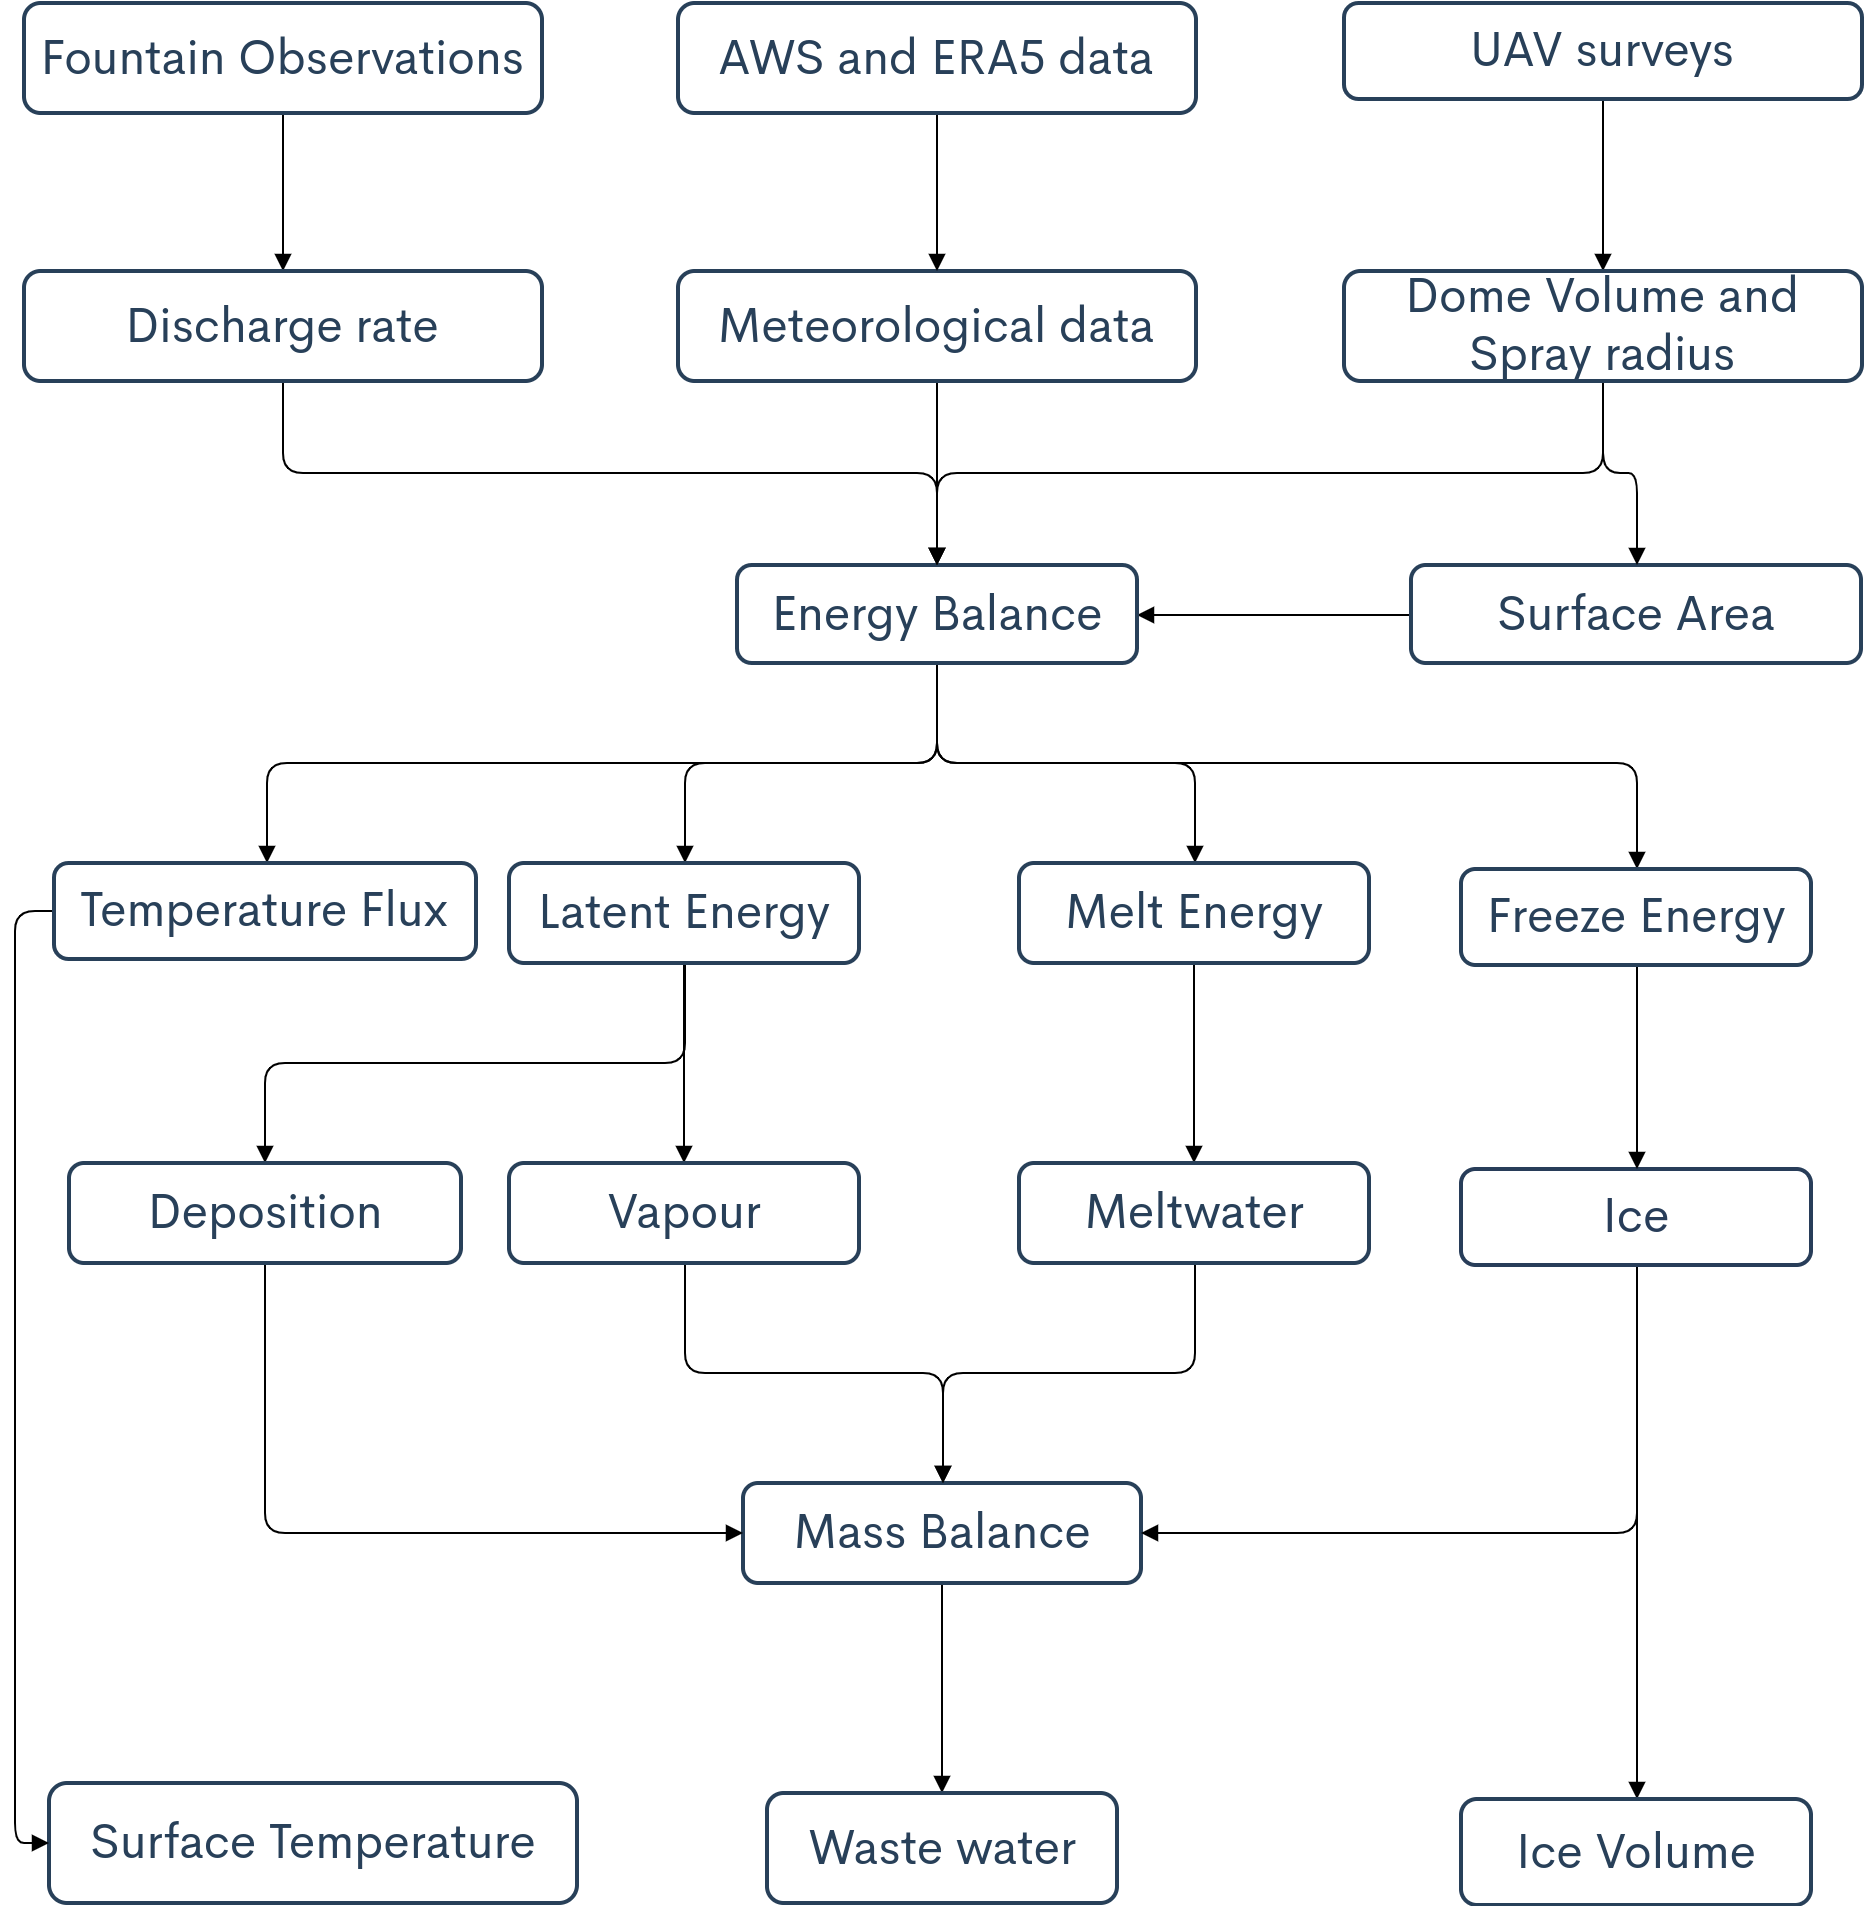
\includegraphics[width=12 cm]{Figures/model_schematic.png} \end{center} \caption{Model
		schematic showing the algorithm used in the model at every time step. } \label{fig:schema} \end{figure}

\subsection{Geometric evolution}

Radius $r_{ice}^i$ and height $h_{ice}^i$ define the dimensions of the AIR assuming its geometry to be a cone. The
surface area $A^i$ and volume $V^i$ are:

\begin{equation} A = A_{corr} \cdot \pi \cdot r_{ice} \cdot \sqrt{{r_{ice}}^2 + {h_{ice}}^ 2} \label{eqn:A} \end{equation}

\begin{equation} V = \pi/3 \cdot {r_{ice}}^2 \cdot h_{ice} \label{eqn:V} \end{equation}

where $A_{corr}$ is a correction factor with values between 1 and 2 that accounts for the increase in surface area
due to the irregular surface of the AIR. We do not specify the time step superscript $i$ of the shape variables
$A$, $V$, $r_{ice}$ and $h_{ice}$. The equations used, display model time step superscript $i$ only if it is
different from the current time step.

With the mass of the AIR $M_{ice}$, its current volume can also be expressed as:

\begin{equation} V = M_{ice} /\rho_{ice} \label{eqn:V1} \end{equation}

where $\rho_{ice}$ is the density of ice (917 $kg\, m^{-3}$).


The influence of the AIR fountain is parameterised by the fountain water temperature $T_{F}$ and its spray radius $r_F$.
The initial radius of the AIR is assumed to be $r_F$. The initial height $h_0$ depends on the dome volume $V_{dome}$
used to construct the AIR as follows:

\begin{equation}
	h_{0} =  \Delta x + \frac{3 \cdot V_{dome}}{\pi r_F^2 }
	\label{eqn:h0}
\end{equation}

where $\Delta x$ is the surface layer thickness (defined in Section \ref{section:EB})

During subsequent time steps, the dimensions of the AIR evolve assuming a uniform ice formation and decay across its
surface area with an invariant slope $s_{cone} = \frac{h_{ice}}{r_{ice}}$ .  During these time steps, the volume is
parameterised using Eqn. \ref{eqn:V} as:

\begin{equation} V = \frac{\pi \cdot {r_{ice}}^3
		\cdot s_{cone}}{3} \label{eqn:V2} \end{equation}


However, the Icestupa cannot outgrow the maximum range of the water droplets ($(r_{ice})_{max} = r_{F}$). Combining
Eqns. \ref{eqn:V},  \ref{eqn:V1}, \ref{eqn:h0} and \ref{eqn:V2}, the geometric evolution of the Icestupa at each time
step $i$ can be determined by considering the following rules:

\begin{equation} (r_{ice},\, h_{ice}) = \left\{ \begin{array}{ll} (r_F ,\, h_0)                                                                        & \textit{ if } i=0 \\
             (r_{ice}^{i-1},\, \frac{3 \cdot M_{ice}}{\pi \cdot \rho_{ice} \cdot {(r_{ice}^{i-1})}^2}) & \textit{ if }
             r_{ice}^{i-1} \geq r_{F} \textit{ and } \Delta M_{ice} > 0                                                    \\ (\frac{3 \cdot M_{ice}}{\pi \cdot \rho_{ice} \cdot s_{cone}})^{1/3} \cdot (1,\,  s_{cone}) &
             otherwise\end{array} \right.  \label{eqn:A2} \end{equation}

where $\Delta M_{ice} = M_{ice}^{i-1} - M_{ice}^{i-2}$

\begin{figure} \begin{center} 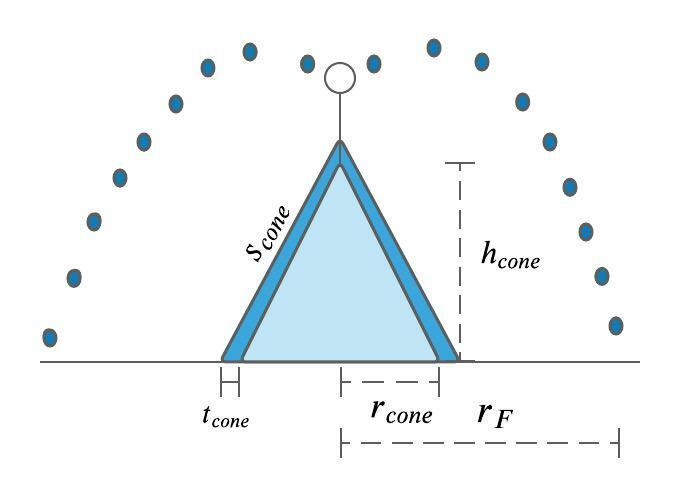
\includegraphics[width=10
			cm]{Figures/shape_parameters.jpeg} \end{center} \caption{Shape variables and fountain constants of the AIR. $r_{ice}$ is
		the radius, $h_{ice}$ is the height and $s_{cone}$ is the slope of the ice cone. $r_F$ is the spray radius, $h_F$ is the
		height and $T_F$ is the water temperature of the fountain.} \label{fig:shape} \end{figure}

\subsection{Energy Balance} \label{section:EB}

The energy balance equation \citep{Hock_2005} for the AIR is formulated as follows:

\begin{equation} q_{surf} = q_{SW} + q_{LW} + q_{L} + q_{S} + q_{F} + q_{G}\label{eqn:EB} \end{equation}

where $q_{surf}$ is the surface energy flux in [$W\,m^{-2}$]; $q_{SW}$ is the net shortwave radiation; $q_{LW}$ is the
net longwave radiation; $q_{L}$ and $q_{S}$ are the turbulent latent and sensible heat fluxes. $q_{F}$ represents the
heat exchange of the fountain water droplets with the AIR ice surface. $q_{G}$ represents ground heat flux between the
AIR surface and its interior. Energy transferred in the direction of the ice surface is always denoted as positive and
away as negative.

Equation \ref{eqn:EB} is usually referred to as the energy budget for “the surface”, but practically it must apply to a
surface layer of ice with a finite thickness $\Delta x$. The energy flux acts upon the AIR surface layer, which has an
upper and a lower boundary defined by the atmosphere and the ice body of the AIR, respectively. The parameter selection
for $\Delta x$ is based on the following two arguments: (a) the ice thickness $\Delta x$ should be small enough to
represent the surface temperature variations every model time step $\Delta t$ and (b) $\Delta x$ should be large enough
for these temperature variations to not reach the bottom of the surface layer. A sensitivity analysis was later
performed to understand the influence of this factor and decide its value. Here, we define the surface temperature
$T_{ice}$ to be the modelled average temperature of the Icestupa surface layer and the energy flux $q_{surf}$ is assumed
to act uniformly across the Icestupa area $A$.

\subsubsection{Net Shortwave Radiation \texorpdfstring{$q_{SW}$}{Lg}}

The net shortwave radiation $q_{SW}$ is computed as follows:
\begin{equation} q_{SW} = (1- \alpha)\cdot (SW_{direct} \cdot f_{cone} + SW_{diffuse}) \label{eqn:SW} \end{equation}

where $SW_{direct}$ and $SW_{diffuse}$ are the ERA5 direct and diffuse shortwave radiation, $\alpha$ is the modelled
albedo and $f_{cone}$ is the area fraction of the ice structure exposed to the direct shortwave radiation.

The albedo varies depending on the water source that formed the current AIR surface layer. During the fountain
occurrence, the albedo assumes a constant value corresponding to ice albedo. However, after the fountain is
switched off, the albedo can reset to snow albedo during snowfall events and then decay back to ice albedo. We use
the scheme described in \cite{OerlemansKnap_1998} to model this process. The scheme records the decay of albedo
with time after fresh snow is deposited on the surface. $\delta t$ records the number of time steps after the last
snowfall event. After snowfall, albedo changes over a time step, $\delta t$ , as

\begin{equation} \alpha=\alpha_{ice}+(\alpha_{snow}-\alpha_{ice}) \cdot e^{(-\delta t)/\tau} \label{eqn:a}
\end{equation}

where $\alpha_{ice}$ is the bare ice albedo value (0.25), $\alpha_{snow}$ is the snow ice albedo value (0.85) and $\tau$
is a decay rate (16 $days$), which determines how fast the albedo of the ageing snow reaches this value.

The area fraction $f_{cone}$ of the ice structure exposed to the direct shortwave radiation depends on the shape
considered. Using the solar elevation angle $\theta_{sun}$, the solar beam can be considered to have a vertical
component, impinging on the horizontal surface (semicircular base of the AIR), and a horizontal component impinging on
the vertical cross section (a triangle). The solar elevation angle $\theta_{sun}$ used is modelled using the
parametrisation proposed by \cite{Woolf_1968}. Accordingly, $f_{cone}$ is determined as follows:

\begin{equation} \begin{split} f_{cone}& =\frac{(0.5 \cdot r_{ice} \cdot h_{ice}) \cdot cos \theta_{sun} +(\pi \cdot
			{r_{ice}}^2/2) \cdot sin \theta_{sun} }{\pi \cdot r_{ice} \cdot ({r_{ice}}^2+{h_{ice}}^2)^{1/2}}\\ \end{split}
	\label{eqn:f_{cone}} \end{equation}

The diffuse shortwave radiation is assumed to impact the conical AIR surface uniformly.

\subsubsection{Net Longwave Radiation \texorpdfstring{$q_{LW}$}{Lg}}

The net longwave radiation $q_{LW}$ is determined as follows:

\begin{equation} q_{LW}= LW_{in}-\sigma \cdot \epsilon_{ice} \cdot {(T_{ice}+ 273.15)}^4
	\label{eqn:LW} \end{equation}

where $T_{ice}$ is the modelled surface temperature, both temperatures are given in [$\degree C$],
$\sigma=5.67\cdot10^{-8}\,Jm^{-2}s^{-1}K^{-4}$ is the Stefan-Boltzmann constant, $LW_{in}$ denotes the incoming longwave
radiation and $\epsilon_{ice}$ is the corresponding emissivity value for the Icestupa surface (0.97).

The incoming longwave radiation $LW_{in}$for the Indian site, where no direct measurements were available, is determined
as follows:

\begin{equation} LW_{in}=\sigma \cdot (\epsilon_a \cdot {(T_a+ 273.15)}^4)
	\label{eqn:LWin} \end{equation}

here $T_a$ represents the measured air temperature and $\epsilon_a$ denotes the atmospheric emissivity. We approximate
atmospheric emissivity $\epsilon_a$ using the equation suggested by \cite{Brutsaert_1982}, considering air temperature
and vapor pressure (Eqn.  \ref{eqn:atm_e}). The vapor pressures over air and ice was obtained using Eqn. \ref{eqn:vp}.
The expression defined in \cite{Brutsaert_1975} for clear skies (first term in equation \ref{eqn:atm_e}) is extended
with the correction for cloudy skies after \cite{Brutsaert_1982} as follows:

\begin{equation} \epsilon_a=1.24 \cdot (\frac{p_{v,a}}{(T_a+273.15)})^{1/7}\cdot(1+0.22\cdot{c}^2) \label{eqn:atm_e}
\end{equation}

with a cloudiness index $c$, ranging from 0 for clear skies to 1 for complete overcast skies. For the Indian site, we
assume cloudiness to be negligible.

\subsubsection{Turbulent fluxes }

The turbulent sensible $q_{S}$ and latent heat $q_{L}$ fluxes are computed with the following expressions proposed by
\cite{Garratt_1992}:

\begin{equation} q_{S}=\mu_{cone}\cdot c_{a} \cdot \rho_{a} \cdot p_{a}/p_{0,a} \cdot \frac{\kappa^2 \cdot v_a \cdot
		(T_a-T_{ice})}{{(\ln{\frac{h_{AWS}}{z_{0}}})}^2} \label{eqn:qs} \end{equation}

\begin{equation} q_{L}=\mu_{cone}\cdot 0.623 \cdot L_s \cdot \rho_{a}/p_{0,a} \cdot \frac{\kappa^2 \cdot
	v_a(p_{v,a}-p_{v,ice})}{{(\ln{\frac{h_{AWS}}{z_{0}}})}^2} \end{equation}

where $h_{AWS}$ is the measurement height above the ground surface of the AWS (around $2\,m$ for all sites), $v_a$ is
the wind speed in [$m\,s^{-1}$], $c_a$ is the specific heat of air at constant pressure (1010 J $kg^{-1} K^{-1}$),
$\rho_{a}$ is the air density at standard sea level (1.29 $kg m^{-3}$), $p_{0,a}$ is the air pressure at standard sea
level (1013 $hPa$), $\kappa$ is the von Karman constant (0.4), $z_{0}$ is the surface roughness (5 $mm$) and $L_s$ is the heat of sublimation (2848 $kJ\,kg^{-1}$).
The vapor pressures over air ($p_{v,a}$) and ice ($p_{v,ice}$) was obtained using the following formulation given in
\cite{WMO_2018}:

\begin{equation} \begin{split} p_{v,a}&=6.107 \cdot 10^{(7.5 \cdot T_a / (T_a + 237.3))}\\ p_{v,ice}&=(1.0016 +
		3.15\cdot10^{-6}\cdot p_{a}-0.074\cdot p_{a}^{-1})\cdot(6.112 \cdot e^{(22.46 \cdot T_{ice} / (T_{ice} + 272.62))})
	\end{split} \label{eqn:vp} \end{equation}

where $p_{a}$ is the measured air pressure in [$hPa$].

The dimensionless parameter $\mu_{cone}$ is an "exposure/roughness parameter" that deals with the fact that AIR has a
rough appearance and forms an obstacle to the wind regime. This factor accounts for the larger turbulent fluxes due to
the roughness of the surface \cite{Oerlemans_2021}, and is a function of the AIR slope as follows:

\begin{equation}
	\mu_{cone} = 1 + \frac{s_{cone}}{2}
\end{equation}


A possible source of error is the fact that wind measurements from the horizontal plane at the AWS are used, which might
be different from those on a slope. However, without detailed datasets from the AIR surface, we retain this assumption.

\subsubsection{Fountain discharge heat flux \texorpdfstring{$q_{F}$}{Lg} }

The fountain water temperature $T_F$ is assumed to cool to 0 $\degree C$. Thus, the heat flux caused by this process is:

\begin{equation}
	q_{F} = \frac{ \Delta M_F \cdot c_{water} \cdot T_F}{\Delta t \cdot A}
	\label{eqn:qF}
\end{equation}
with $c_{water}$ as the specific heat of water.

\subsubsection{Bulk Icestupa heat flux \texorpdfstring{$q_{G}$}{Lg}} \label{sec:Bulkflux}

The bulk Icestupa heat flux $q_{G}$ corresponds to the ground heat flux in normal soils and is caused by the temperature
gradient between the surface layer ($T_{ice}$) and the ice body ($T_{bulk}$). It is expressed by using the heat
conduction equation as follows:

\begin{equation} q_{G} = k_{ice} \cdot (T_{bulk}-T_{ice}^{i-1})/l_{ice} \label{eqn:qG}    \end{equation}

where $k_{ice}$ is the thermal conductivity of ice (2.123 $W\, m^{-1}\,K^{-1}$) , $T_{bulk}$ is the mean temperature of
the ice body within the Icestupa and $l_{ice}$ is the average distance of any point in the surface to any other point in
the ice body. $T_{bulk}$ is initialised as 0 $\degree C$ and later determined from Eqn. \ref{eqn:qG} as follows:

\begin{equation} T_{bulk}^{i+1} = T_{bulk} - (q_{G} \cdot A \cdot \Delta t)/(M_{ice} \cdot c_{ice}) \end{equation}

Since AIRs typically have conical shapes with $r_{ice} > h_{ice}$, we assume that the center of mass of the ice body is
near the base of the fountain. Thus, the distance of every point in the AIR surface layer from the ice body's center of
mass is between $h_{ice}$ and $r_{ice}$. We calculate $q_{G}$ assuming $l_{ice} = (r_{ice} + h_{ice})/2$.


\subsection{Surface temperature}

The available energy $q_{surf}$ can act on the surface of the AIR to a) change its temperature, b) melt ice or c) freeze
ice.

So Eqn. \ref{eqn:EB} can be rewritten as: \begin{equation} q_{surf} = q_{freeze/melt} + q_{T} \end{equation} where
$q_{T}$, $q_{freeze}$ and $q_{melt}$ represent energy associated with process (a), (b) and (c) respectively.

We categorize the model time steps as freezing or melting events to distribute the surface energy flux into these three
components. Freezing/Melting events can only occur, if fountain water is available and the surface energy flux is
negative/positive. However, these two conditions are not sufficient as the latent heat energy can only contribute to
temperature fluctuations. Therefore, preventing latent heat energy from turning a melting event into a freezing event an
additional condition namely $(q_{surf}-q_{L}) < 0$ is required.

\begin{equation}
	q_{freeze/melt} = \left\{ \begin{array}{ll}
		q_{freeze} & \textit{ if } \Delta M_{F} > 0 \textit{ and } q_{surf} < 0 \textit{ and }(q_{surf}-q_{L}) < 0 \\
		q_{melt}   & \textit{ otherwise}
	\end{array} \right.
\end{equation}

During a freezing event, the AIR surface is assumed to warm to $0 \degree C$. The available energy $(q_{surf}-q_{L})$ is
further augmented due to this change in surface temperature represented by the energy flux $q_{0} = \frac{\rho_{ice}
		\cdot \Delta x \cdot c_{ice} \cdot T_{ice}^{i-1}}{\Delta t}$. The available energy can either be sufficient or
insufficient to freeze the fountain water available. If insufficient, the additional energy further cools down the
surface temperature. The surface energy flux distribution during a freezing event can be represented as:

\begin{equation}
	(q_{freeze}, q_{T}) = \left\{ \begin{array}{ll}
		(q_{surf}-q_{L}+q_{0}, q_{L}-q_{0}) & \textit{ if } \Delta M_{F} \geq -\frac{(q_{surf}-q_{L}+q_{0}) \cdot A \cdot \Delta
		t}{L_f}                                                                                                                  \\
		(\frac{\Delta M_{F} \cdot L_f
		}{A \cdot \Delta t}
		, q_{surf}+\frac{\Delta M_{F} \cdot L_f
		}{A \cdot \Delta t})                & \textit{ if } \Delta M_{F} < -\frac{(q_{surf}-q_{L}+q_0) A \cdot \Delta
		t}{L_f}
	\end{array} \right.
\end{equation}

During a melting event, the surface energy flux ($q_{surf}$) is first used to change the surface temperature to
$T_{temp}$ calculated as:

\begin{equation} T_{temp} =\frac{q_{surf} \cdot \Delta t}{\rho_{ice} \cdot c_{ice} \cdot \Delta x} + T_{ice} \end{equation}

If $T_{temp} > 0 \degree C$, then energy is reallocated from $q_{T}$ to $q_{melt}$ to maintain surface temperature at
melting point. The surface energy flux distribution during a melting event can be represented as:

\begin{equation}
	(q_{melt}, q_{T}) = \left\{ \begin{array}{ll}
		(0, q_{surf})                                                                                                                                                 & \textit{ if } T_{temp} < 0 \\
		(\frac{T_{temp} \cdot \rho_{ice} \cdot c_{ice} \cdot \Delta x}{\Delta t}, q_{surf}-\frac{T_{temp} \cdot \rho_{ice} \cdot c_{ice} \cdot \Delta x}{\Delta t}  ) & \textit{ if } T_{temp} > 0
	\end{array} \right.
\end{equation}


\subsection{Mass Balance}

The mass balance equation for an AIR is represented as:

\begin{equation}
	\frac{\Delta M_{F} + \Delta M_{ppt} + \Delta M_{dep}}{\Delta t} = \frac{\Delta M_{ice} +\Delta M_{water} +
		\Delta M_{sub} + \Delta M_{runoff}}{\Delta t}  \\
	\label{eq:MB}
\end{equation}

where $M_{F}$ is the discharge of the fountain; $M_{ppt}$ is the cumulative precipitation;  $M_{dep}$ is the cumulative
accumulation through water vapour deposition; $M_{ice}$ is the cumulative mass of ice; $M_{water}$ is the cumulative
mass of melt water; $M_{sub}$ represents the cumulative water vapor loss by sublimation and $M_{runoff}$ represents the
fountain discharge runoff that did not interact with the AIR. The LHS of equation \ref{eq:MB} represents the rate of
mass input and the RHS represents the rate of mass output for an AIR.

Precipitation input is calculated as shown in equation \ref{eq:ppt} where $\rho_{w}$ is the density of water (1000
$kg\,m^{-3}$), $ppt$ is the measured precipitation rate in [$m\,s^{-1}$] and $T_{ppt}$ is the temperature threshold
below which precipitation falls as snow. Here, snowfall events were identified using $T_{ppt}$ as $1 \degree C$. Snow
mass input is calculated by assuming a uniform deposition over the entire circular footprint of the AIR.

The latent heat flux is used to estimate either the evaporation and condensation processes or sublimation and deposition
processes as shown in equation \ref{eq:vap}. During time steps at which surface temperature is below 0 $\degree C$ only
sublimation and deposition can occur, but if the surface temperature reaches 0 $\degree C$, evaporation and condensation
can also occur. As the differentiation between evaporation and sublimation (and condensation and deposition) when the
air temperature reaches 0 $\degree C$ is challenging, we assume that negative (positive) latent heat fluxes correspond
only to sublimation (deposition), i.e. no evaporation (condensation) is calculated.

Since we have categorized every time step as a freezing and melting event, we can determine the meltwater and  ice
generated using the associated energy fluxes as shown in equations \ref{eq:mwat} and \ref{eq:mice}. Having calculated
all the other mass components the fountain wastewater generated every time step can be calculated using Eqn.
\ref{eq:MB}.

\begin{subequations}
	\label{equations}
	\begin{align}
		\label{eq:ppt}
		\frac{\Delta M_{ppt}}{\Delta t}                                    & = \left\{ \begin{array}{ll} \pi \cdot {r_{ice}}^2 \cdot
			\rho_{w}\cdot ppt & \textit{ if } T_{a} < T_{ppt} \\ 0 & \textit{ if } T_{a} \geq T_{ppt} \\\end{array} \right.                                      \\
		\label{eq:vap}
		(\frac{\Delta M_{dep}}{\Delta t}, \frac{\Delta M_{sub}}{\Delta t}) & = \left\{ \begin{array}{ll} \frac{q_{L}
			\cdot A}{L_s}\cdot (1,0)  & \textit{ if } q_{L} \geq 0 \\ \frac{q_{L}
			\cdot A}{L_s}\cdot (0,-1) & \textit{ if } q_{L} < 0    \\\end{array} \right.                                      \\
		\label{eq:mwat}
		\frac{\Delta M_{water}}{\Delta t}                                  & = \frac{q_{melt} \cdot A }{L_f}                                                   \\
		\label{eq:mice}
		\frac{\Delta M_{ice}}{\Delta t}                                    & = \frac{q_{freeze}\cdot A }{L_f} + \frac{\Delta M_{ppt}}{\Delta t} + \frac{\Delta
			M_{dep}}{\Delta t}- \frac{\Delta M_{sub}}{\Delta t}- \frac{\Delta M_{melt}}{\Delta t}
	\end{align}
\end{subequations}

We define the freezing rate $m_{freeze}$ and the melting rate $m_{melt}$ as follows:

\begin{equation}
	m_{freeze/melt} = \frac{q_{freeze/melt} \cdot A }{L_f}
\end{equation}

To estimate the mass of any component at time step $i$, one can now sum the mass flux estimated above: \begin{equation}
	M_{comp}^i = \sum_{t=0}^{t=i} (\frac{\Delta M_{comp}}{\Delta t})_{t} + M_{comp}^0 \end{equation} where

\begin{equation} M_{comp}^0 = \left\{ \begin{array}{ll} -V_{dome} * \rho_{ice} & \textit{ if } M_{comp}=
             M_{ice}\textit{ or }
             M_{F}                                                 \\ 0 & \textit{ otherwise }\\\end{array} \right. \\
\end{equation}

Considering AIRs as water reservoirs, their storage efficiency ($SE$) can be defined as the percentage of ice and
meltwater produced as follows:

\begin{equation} \textit{SE} = \frac{M_{water}+M_{ice}}{(M_F+M_{ppt}+M_{dep})} \cdot 100 \end{equation}

\subsection{Sensitivity and uncertainty analysis}

We used a polynomial chaos expansion approach (as in \cite{uncertainpy_2018}; \cite{Xiu_2005}) to evaluate the
model sensitivity and uncertainty.  Polynomial chaos expansion are a much more efficient way to obtain similar
results compared to the computationally demanding Monte Carlo methods. This approach approximates the model with a
polynomial (as a surrogate model), on which sensitivity and uncertainty analysis can be performed.  The surrogate
model produced was a polynomial of order 4. The rosenblatt transformation was also used since the parameters were
correlated.

The uncertainty in the model ice volume estimates are caused due to uncertainty in two sources, namely model
parameters and input. For the model parameters, we first fix a range based on literature values and then perform a
global sensitivity analysis (GSA) with the storage efficiency as the objective. The distribution is always treated
as uniform and the limits for every parameter are given in Table \ref{tab:parameters}. The GSA consists of a total
ensemble size of 2000 simulations per AIR. The parameter sensitivity results from the GSA are used as a tool to
reduce the number of free parameters in the model by identifying those parameters which have only a marginal
influence on the model output. The model is considered insensitive to parameters with a total sensitivity index
($S_{T_{i}}$) of $\leq 0.05$, and these parameters were fixed at the median value of the range shown in Table
\ref{tab:parameters} in subsequent model simulations.

The ranges for the snow albedo were taken from \cite{ZollesMaussion_2019}; ice albedo minimum was taken from
\cite{steiner_2015} and maximum from \cite{ZollesMaussion_2019}; albedo decay rate is assumed to have a minimum
value of 10 days similar to values obtained by \cite{Schmidt_2017} for wet surfaces and a maximum of 22 days from
\cite{OerlemansKnap_1998}; emissivity range from \cite{steiner_2015} and temperature threshold for precipitation
from \cite{Zhou_2010}. The surface area correction factor, $A_{corr}$, quantifies the deviation of the AIR shape
from the conical shape assumed in the model. We assume the range of this deviation to be between 1 to 2. Literature
values for surface roughness, $z_{0}$, of glacier ice are generally in the range $0.1-5\, mm$
\citet{BrockWillisSharp_2006}. Since the surface layer thickness, $\Delta x$, for an AIR does not bear resemblance
to any parameter in the glaciological literature, we attribute a wide range of values for it and try to constrain
it further during the calibration process.

For the model input data, uncertainty associated with two kinds of observations namely, weather and fountain were
evaluated. All the radiation measurements ($SW_{direct}, SW_{diffuse}, LW_{in}$) in the weather data were uncertain
since they were taken from ERA5 dataset or an AWS far away from the AIR site. All the measured fountain parameters are
uncertain since they vary significantly temporally and are not constant. The UAV measurements have also uncertainty
associated with them. So all these measurements were assumed to have an uncertainty of $\pm 10 \%$ to evaluate the
corresponding uncertainty produced in model ice volume estimates.

The sensitivity analysis was only carried out for the CH21 and IN21 AIR since CH20 AIR had too few ice volume
observations for calibration.

\begin{table}
	\centering
	\caption{The ranges of the 8 different parameters used in the sensitivity study.}
	\label{tab:parameters}
	\begin{tabular}{@{}llllll@{}}
		\toprule
		\textbf{No.} & \textbf{Name}                       & \textbf{Abbreviation} & \textbf{Min} & \textbf{Max} & \textbf{Unit} \\\midrule
		1            & Ice Emissivity                      & $\epsilon_{ice}$      & 0.95         & 0.99         &               \\
		2            & Ice Albedo                          & $\alpha_{ice}$        & 0.15         & 0.35         &               \\
		3            & Snow Albedo                         & $\alpha_{snow}$       & 0.8          & 0.9          &               \\
		4            & Precipitation Temperature threshold & $T_{ppt}$             & 0            & 2            & $\degree C$   \\
		5            & Albedo Decay Rate                   & $\tau$                & 10           & 22           & $days$        \\
		6            & Surface Roughness                   & $z_0$                 & 1            & 5            & $mm$          \\
		7            & Surface Area correction factor      & $A_{corr}$            & 1            & 2            &               \\
		8            & Surface layer thickness             & $\Delta x$            & 10           & 50           & $mm$          \\\bottomrule
	\end{tabular}
\end{table}

\section{Results}

\subsection{Sensitivity and uncertainty analysis}

The focus of the GSA is not on the absolute sensitivity towards single parameters, but rather to reduce the dimension
of the parameter space. Therefore, the following discussion is limited to two classes: parameters to which the model is
sensitive ($S_{T_{i}} > 0.05$) and non-sensitive ($S_{T_{i}} \leq 0.05$).

For all the AIR, most of the parameters related to the albedo module were insensitive namely, $\alpha_{snow}$,
$\tau$ and $T_{ppt}$. This is to be expected since albedo is forced to be the ice albedo during fountain runtime,
these parameters are only used for roughly half the model duration and only if there is any precipitation. We end
up with only 5 out of the 8 free parameters that need to be calibrated further.

Model simulations were carried out varying all the sensitive parameters within the ranges defined in Table
\ref{tab:parameters}. The model performance was expressed by the RMSE determined between the UAV ice volume
observations and the model ice volume outputs. Fig.  \ref{fig:param_hist} shows the frequency distribution of the
sensitive parameters among the best 100 runs from a total of 2500 model runs for each AIR.

\begin{figure}
	\begin{center}
		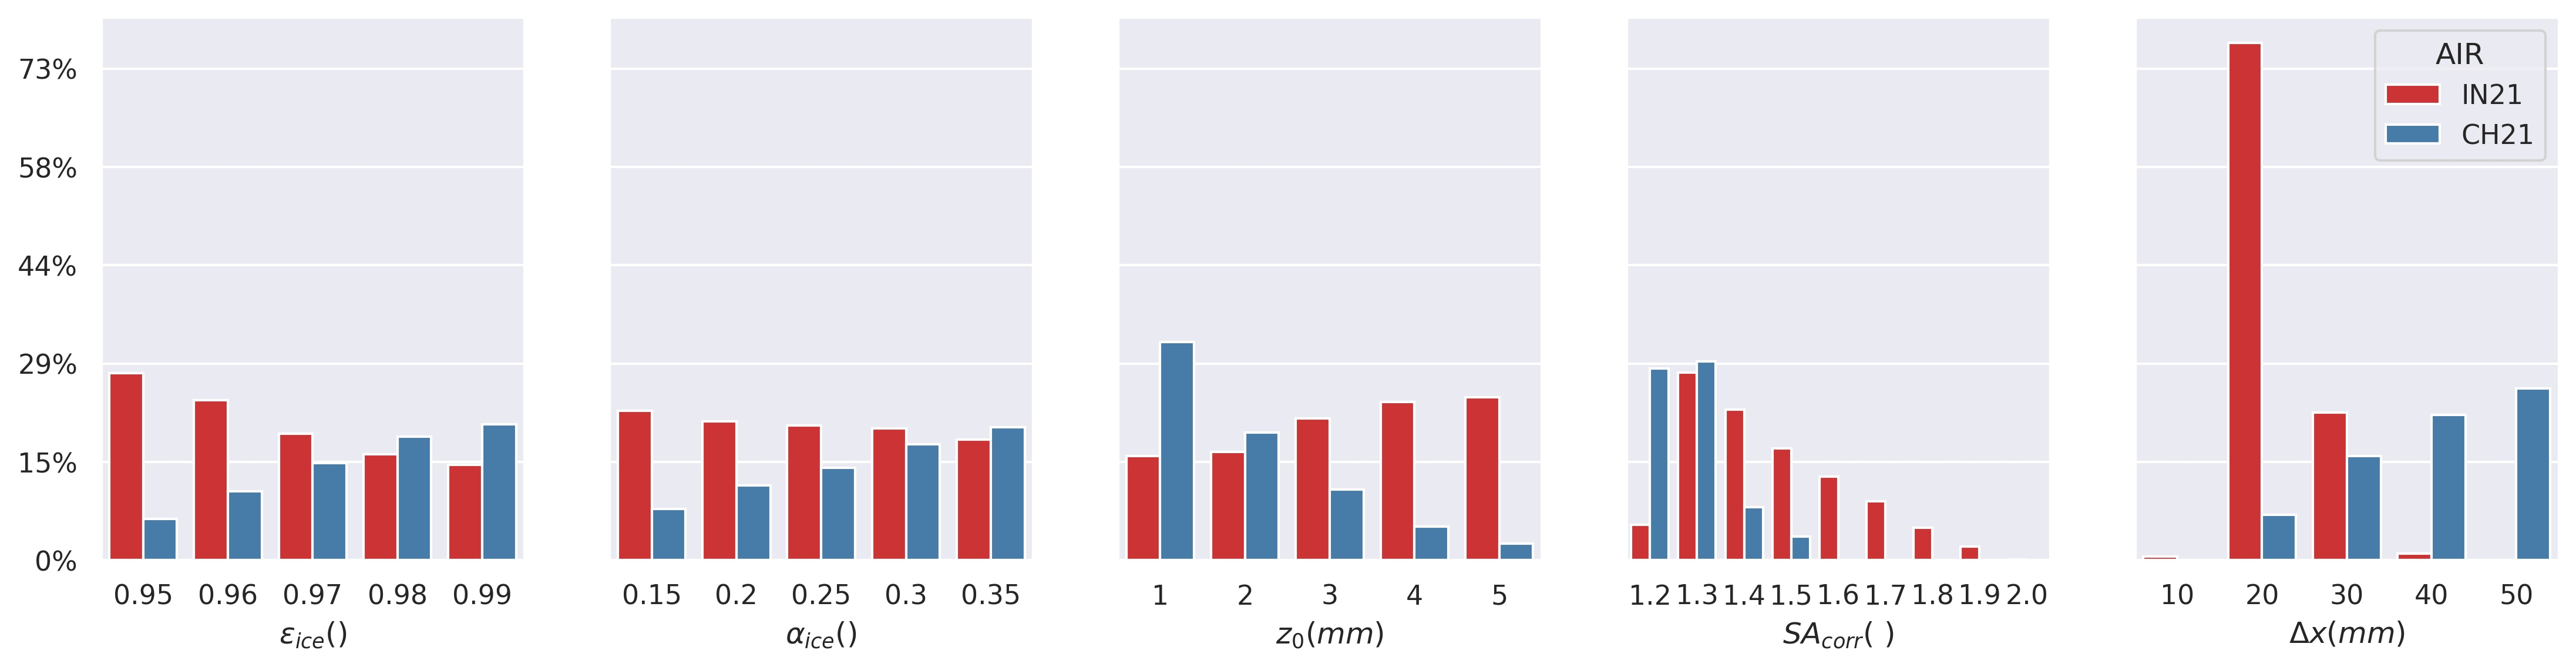
\includegraphics[width=\linewidth]{Figures/param_hist.jpg}
	\end{center}
	\caption{Observed ranges of the sensitive parameters used in the model optimization, shown by
		plotting the frequency distribution of the parameter values for the best 100 of the model runs. }
	\label{fig:param_hist} \end{figure}

In general, none of the sensitive parameters exhibit significant preference to any value in their ranges.  However,
IN21 AIR does exhibit a strong preference for a surface layer thickness of $20\,mm$. Hence, this model parameter
was calibrated as such for all the AIR and the rest of the parameters were calibrated to their median values.

The uncertainty in the ice volume estimates caused by the model parameters and input are shown in Fig.
\ref{fig:results}.

\begin{figure}
	\begin{center}
		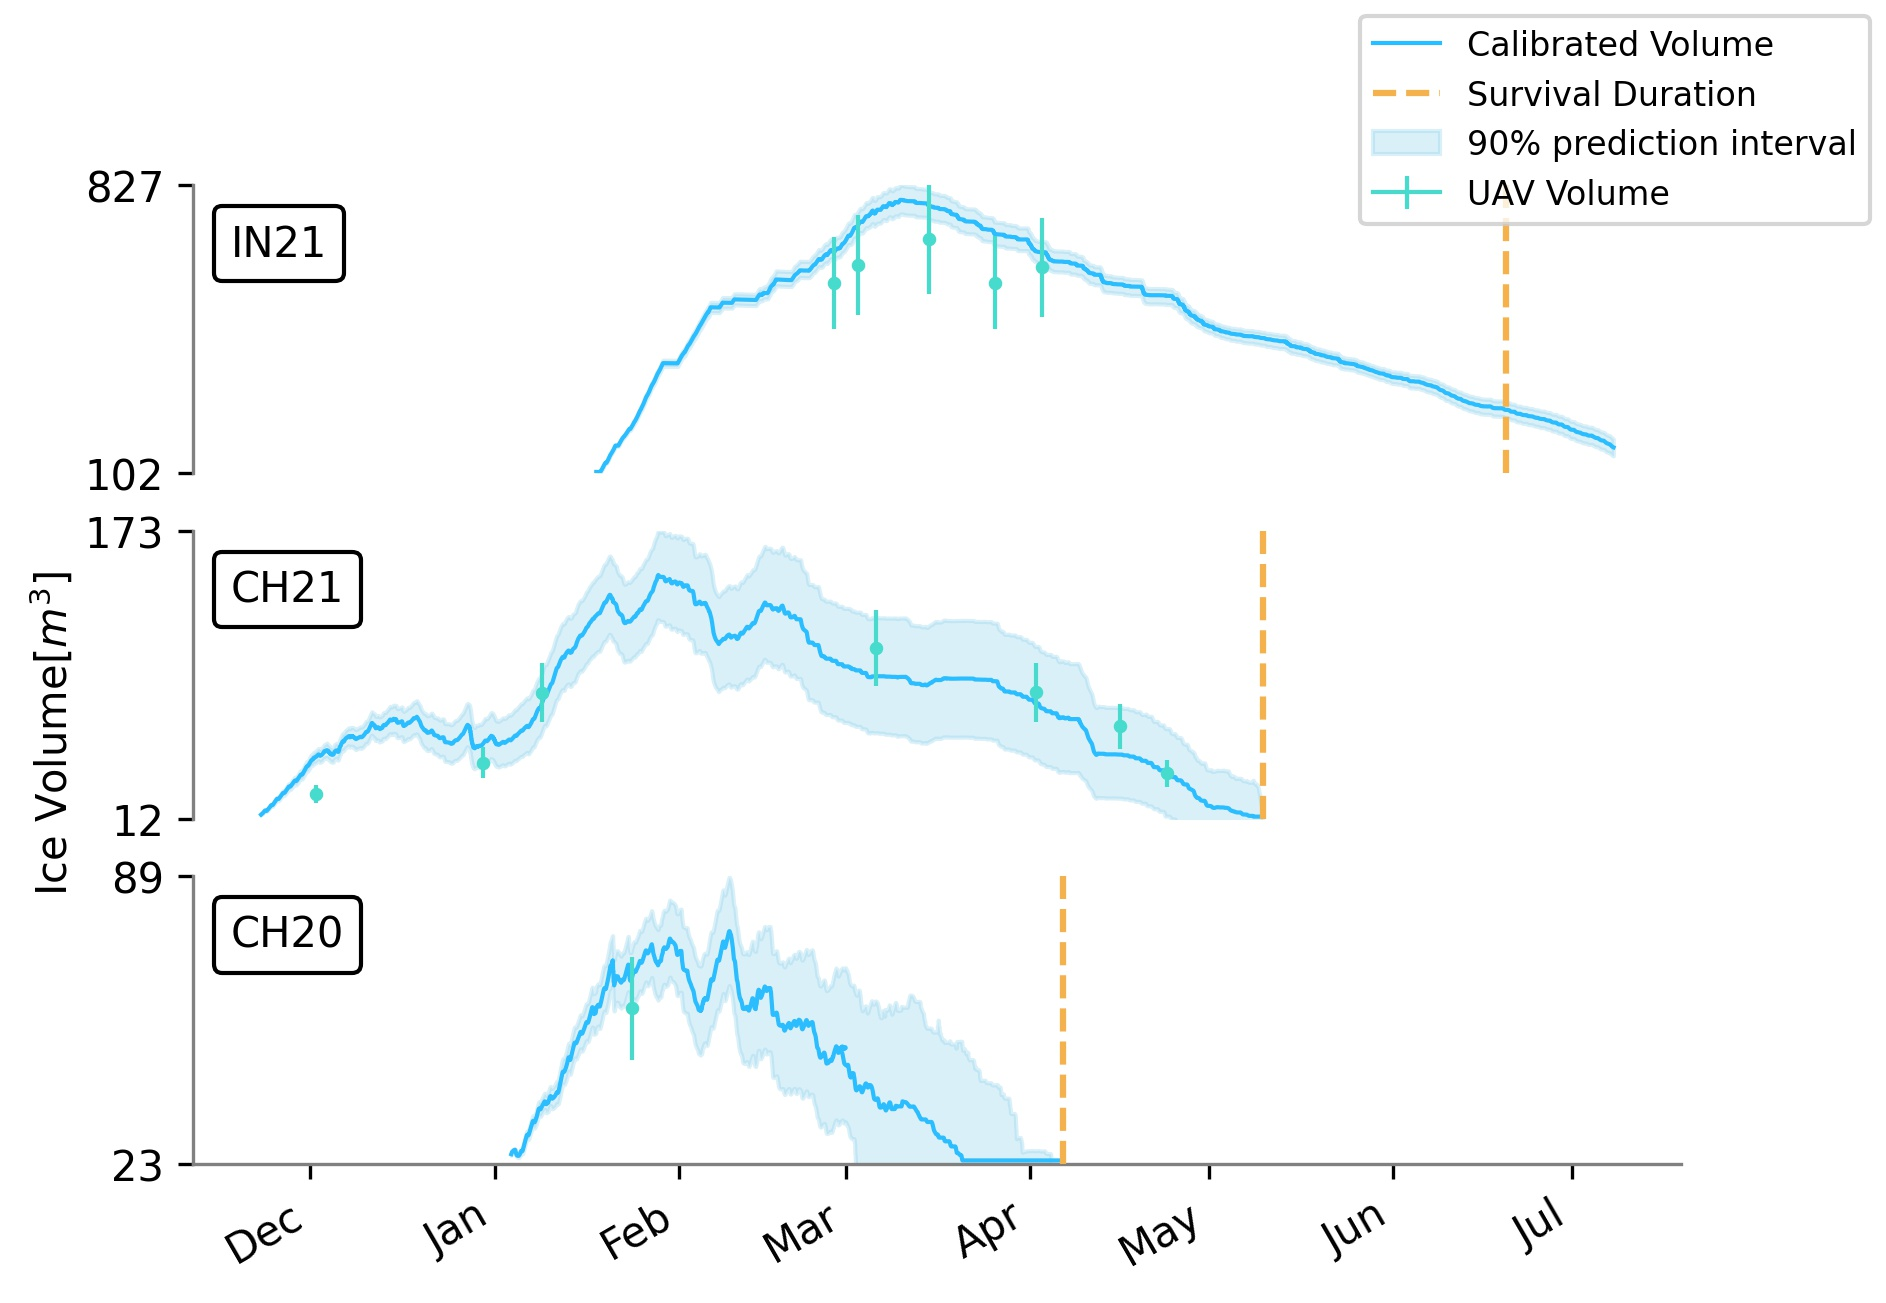
\includegraphics[width=\linewidth]{Figures/icev_results.jpg}
	\end{center}
	\caption{Modelled ice volume during the lifetime of the AIR (blue curve). Green points indicate the validation
		measurements. The prediction interval is based on the ice volume uncertainty caused by the significant parameters.  The
		upper and lower bounds of the y axis represents maximum ice volume and dome volume respectively.  }
	\label{fig:results} \end{figure}


\subsection{AIR ice volume estimates}

The construction decisions responsible for the observed magnitude and variance of the ice volume estimates shown in
Fig. \ref{fig:results} can be categorised based on the the fountain used and location chosen. The construction
location chosen determines the weather and the fountain usage determines the surface area through its spray radius.
To isolate the influence of the fountain and location, we further divide the ice volume estimates into the daily
surface normal thickness change (mass flux) and the energy flux respectively. Fig. \ref{fig:MEB} shows these daily
fluxes calculated with calibrated parameters for the first and last 20 days for each AIR. The two time periods
selected are characteristic of the freezing and melting period respectively. A strong variability is evident
between the freezing and melting periods and between the Swiss and the Indian AIR.

The magnitude of the mass fluxes in Fig. \ref{fig:MEB} are explained by their energy flux counterparts. Namely ice
mass flux corresponds to freezing energy available, melt mass flux corresponds to melting energy available,
snowfall is calculated directly form the precipitation quantity and ice radius and sublimation/deposition
quantities correspond to the latent heat flux available. The rest of the energy fluxes are shown to represent the
different physical processes that contribute to this freezing and melting energy.

\subsubsection{Location influence}


To understand the location influence, we compare the Swiss and the Indian AIR during the melting period. The mass
and energy fluxes show how the surface thickness of both the AIR was lost mostly due to sensible heat flux. The
Indian AIR melted gradually but the Swiss AIR melted rapidly on certain days (e.g. day 140) due to foehn events
which increased the wind speed and air temperature drastically.

Latent heat plays a fascinating role in this whole energy balance. It contributes to both mass and energy flux
simultaneously through deposition/sublimation processes. Since the heat of vaporization is large, sublimation
(deposition) process can contribute significantly to the freezing (melting) energy without affecting the overall
mass flux much. This can be observed throughout the life cycle of the Indian AIR, where sublimation either
contributed to more ice mass or compensated the sensible heat flux during the freezing and melting period,
respectively. Sublimation was significantly greater in the Indian site compared to the Swiss site as the
corresponding latent heat fluxes were an order of magnitude larger (see Table \ref{tab:Observations}). This was
primarily due to the difference in relative humidity between the sites.

Longwave radiation compensates the shortwave radiation to a large degree during the melting period for both the
locations.

\begin{figure}
	\begin{center}
		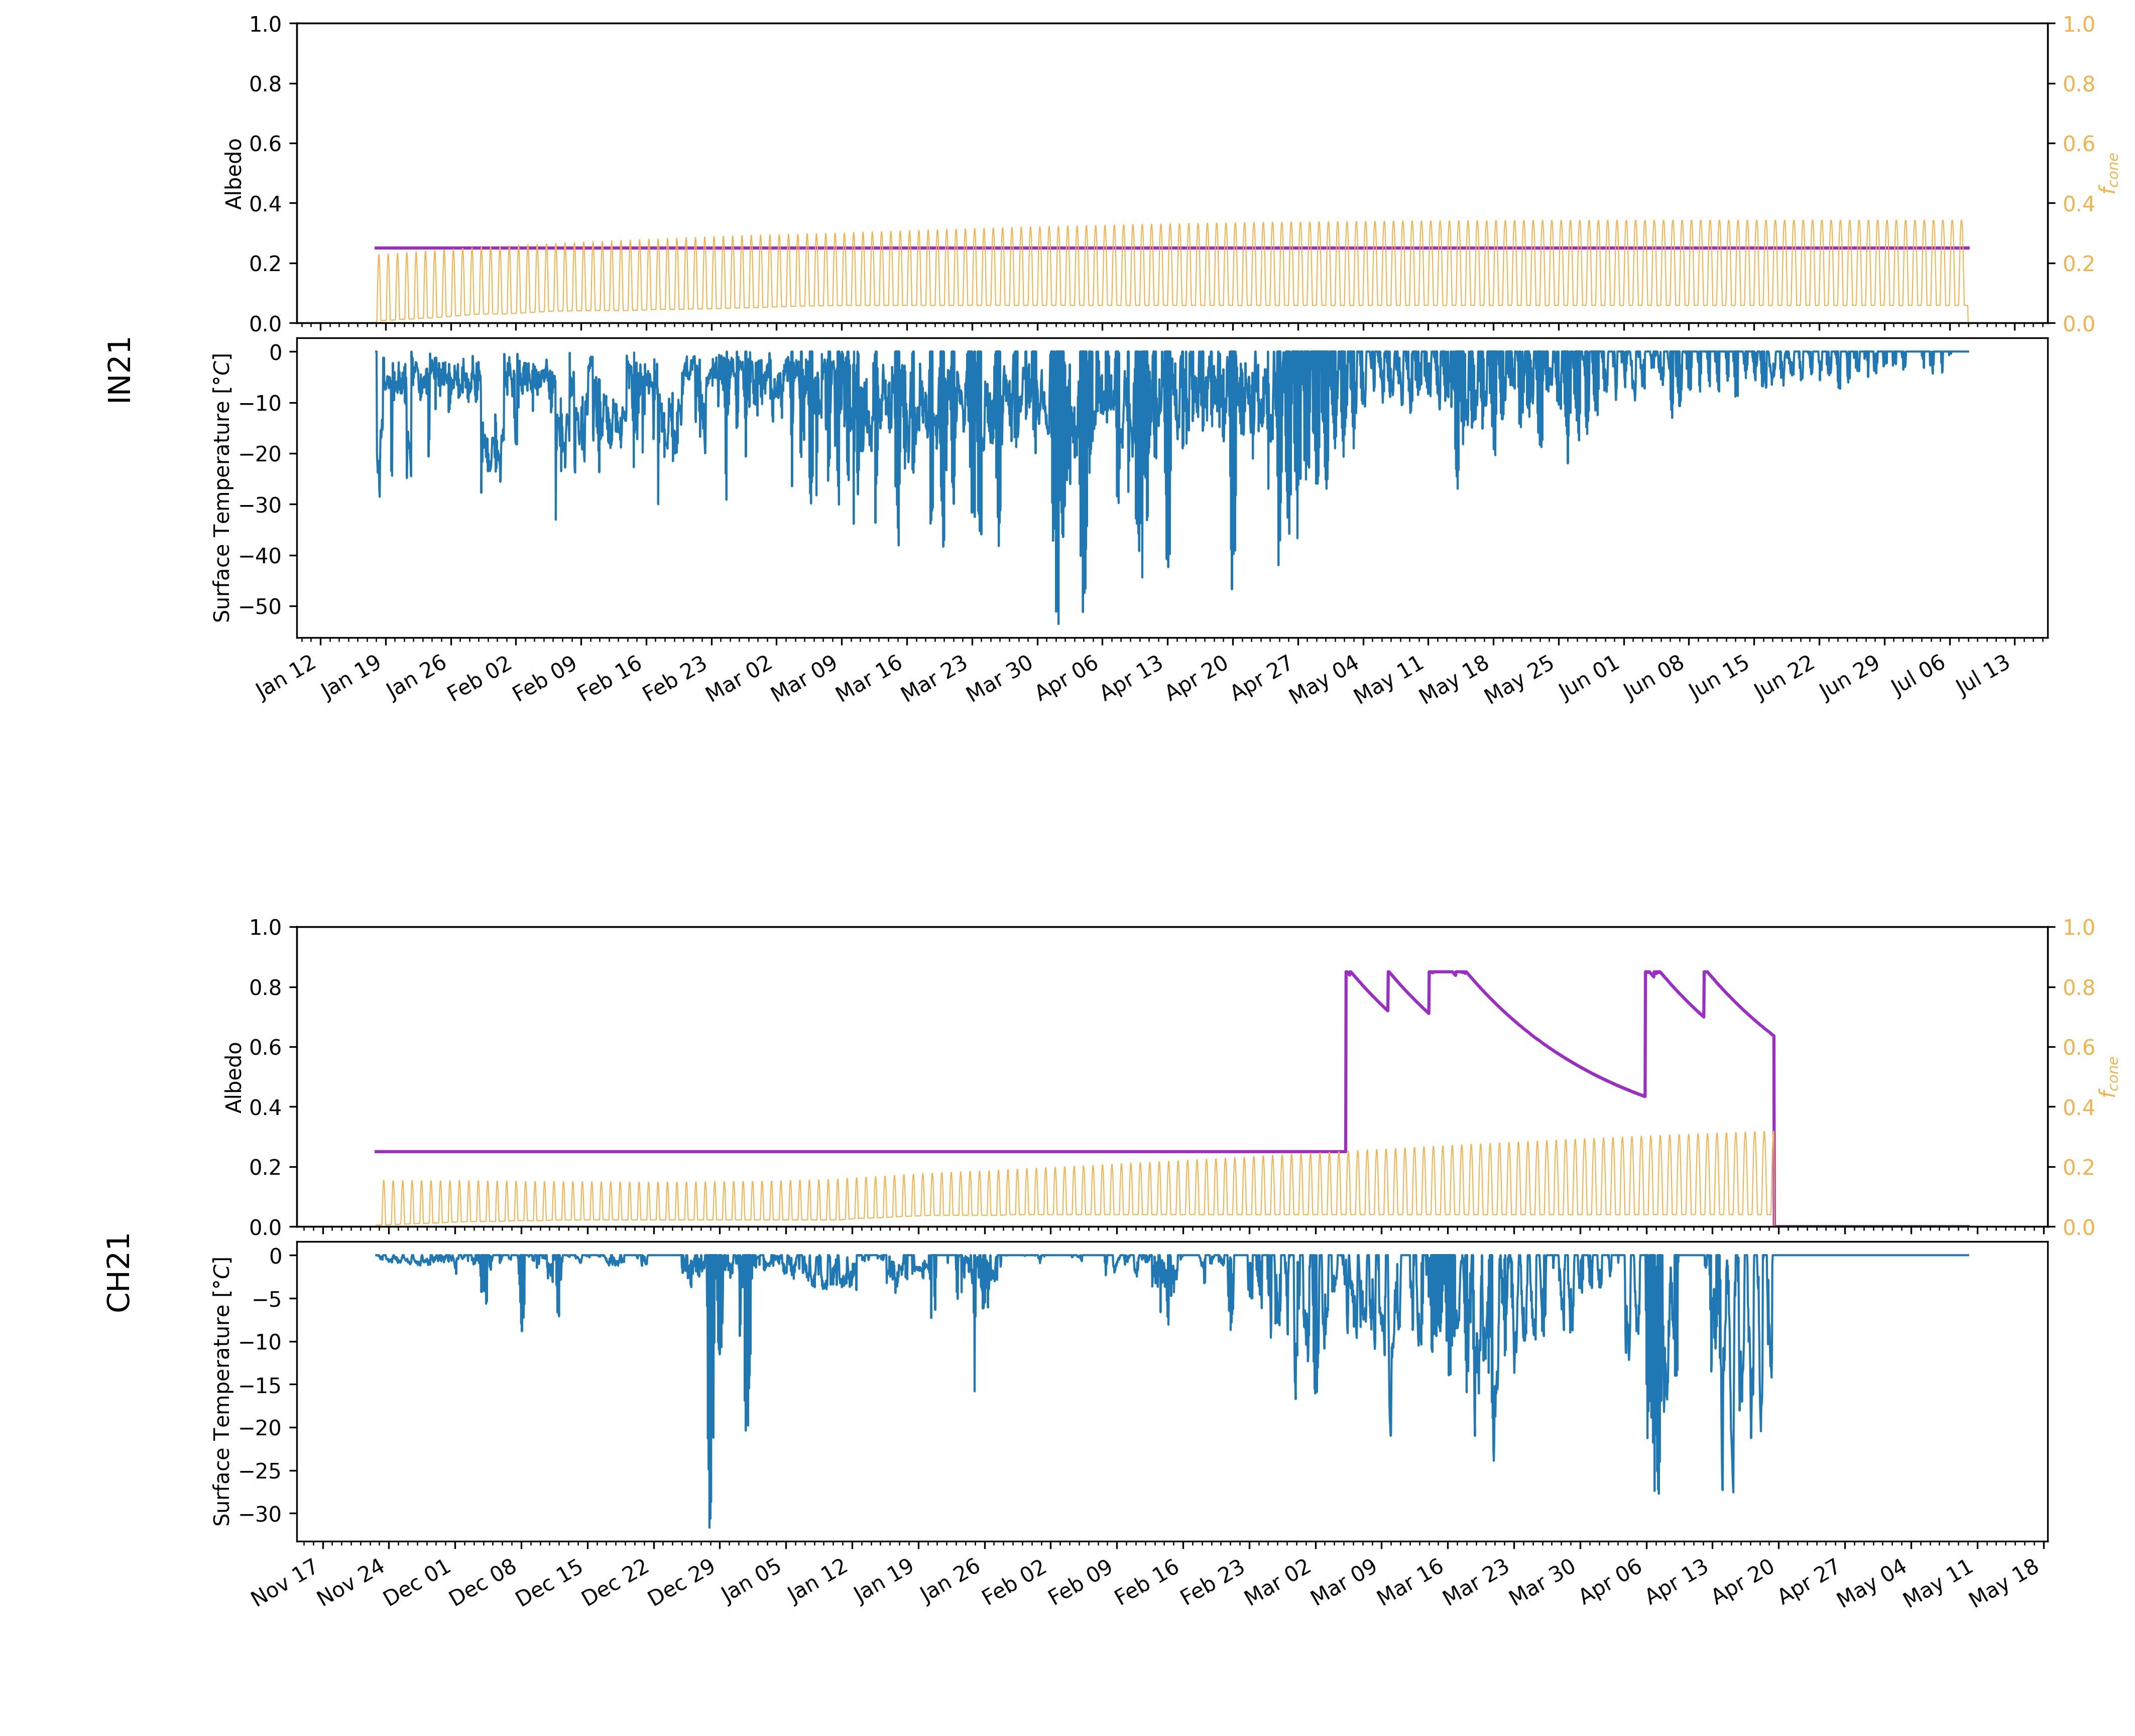
\includegraphics[width=\linewidth]{Figures/albedo.jpg}
	\end{center}
	\caption{Some derived parameters of the model, namely, albedo and $f_{cone}$ (a), Surface temperature (b). In
		(a), the purple curve shows how snow and fountain spray reset albedo between ice albedo and snow albedo.  The
		decay of the snow albedo to ice albedo can also be observed. The orange curve shows how the solar radiation area
		fraction varied diurnally and seasonally with variations in the solar elevation angle. In (b), the surface
		temperature (blue curve) was forced to be 0 $\degree C$ during fountain runtime.}
	\label{fig:albedo}
\end{figure}

Direct shortwave radiation is more than 3 times higher for the Indian location (due to its higher altitude) but
there is no significant difference in the net shortwave radiation absorbed by both the AIR. This is because of the
higher diffuse shortwave radiation in the Swiss location compensates for its lower direct shortwave radiation
(Table \ref{tab:Observations}).  Since the Indian location has mostly clear days, its diffuse shortwave radiation was
negligible. Moreover, the effect of the direct shortwave radiation of both the locations was dampened by the area
fraction $f_{cone}$. As shown in Fig. \ref{fig:albedo}, less than half of the AIR surface area was exposed to
direct shortwave radiation flux.  Albedo, on the other hand, only varied for the Swiss location since there was
negligible precipitation for the Indian site.

\begin{figure}
	\begin{center}
		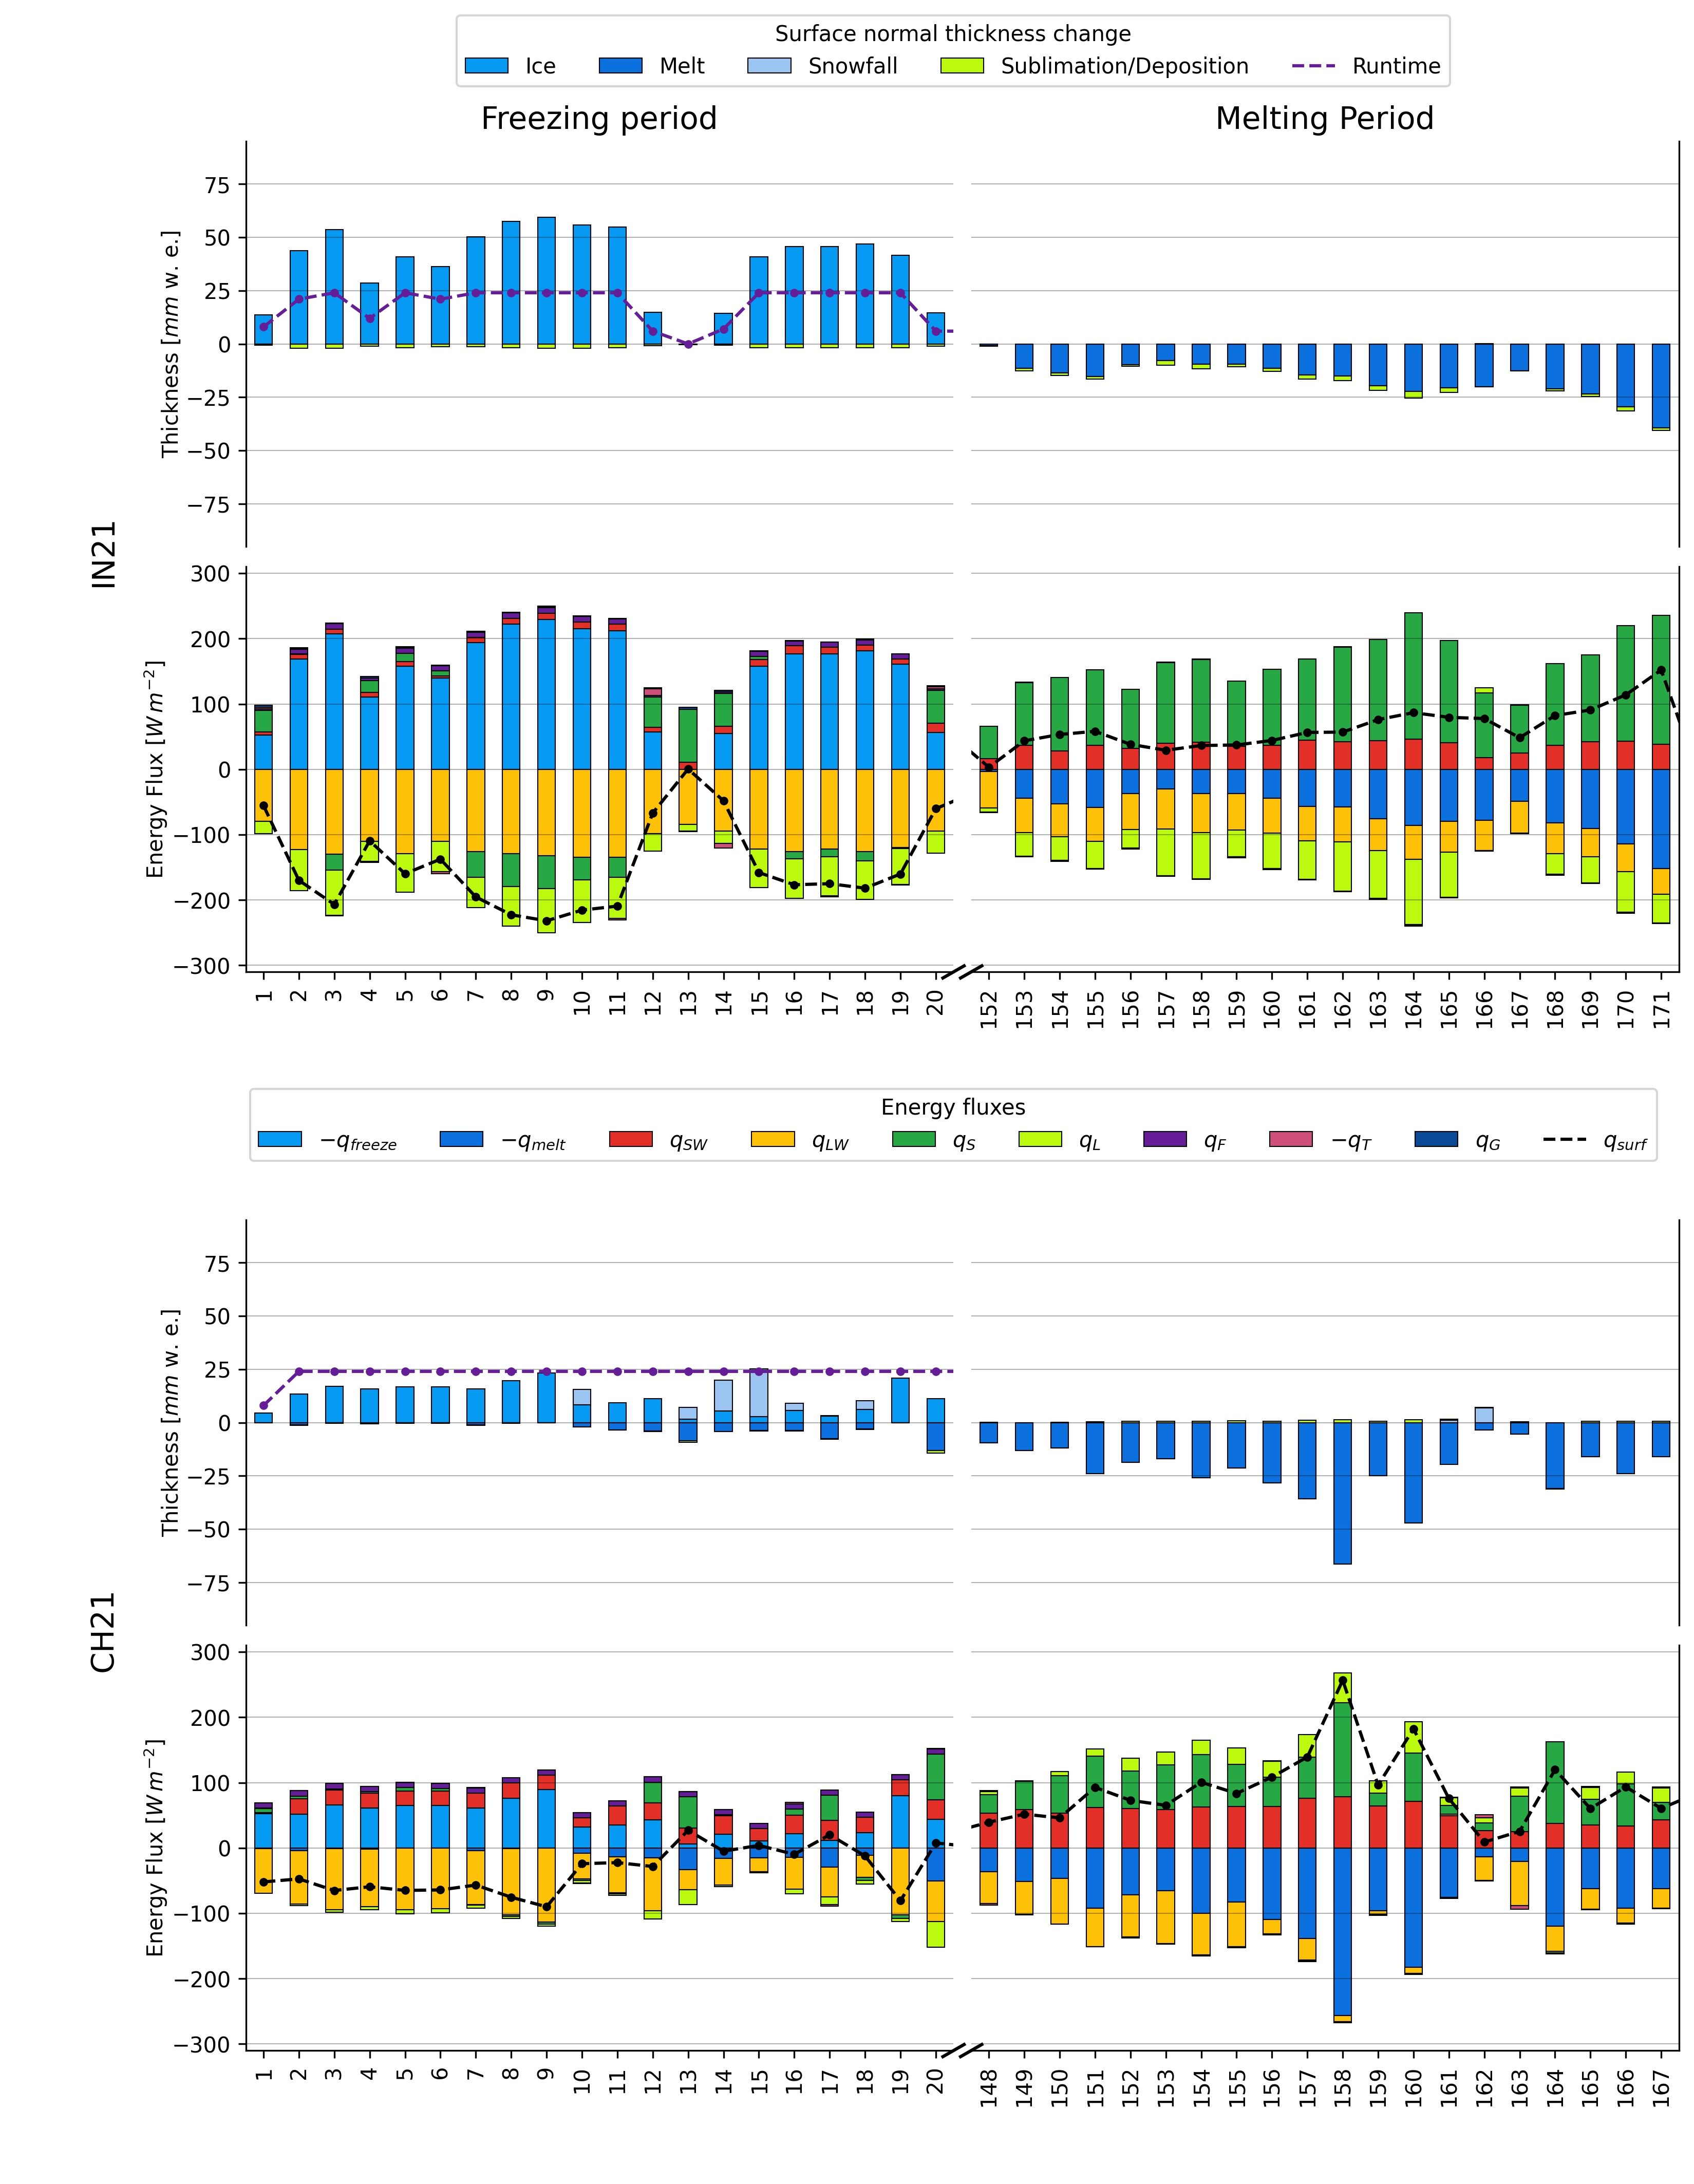
\includegraphics[width=\linewidth]{Figures/mass_energy_bal.jpg} \end{center}
	\caption{Daily averages of mass and energy fluxes compared for all AIRs during their freezing and melting periods.
	} \label{fig:MEB}
\end{figure}


\begin{table}
	\centering
	\caption{ Summary of the mass balance, energy balance and AIR characteristics estimated by the model}
	\label{tab:Results}
	\begin{tabular}{@{}|lllll|@{}}
		\toprule
		\textbf{}              & \textbf{Name}           & \textbf{Symbol}           & \textbf{IN21} & \textbf{CH21} \\ \midrule
		\multicolumn{1}{|l|}{\multirow{3}{*}{\rotatebox[origin=c]{90}{Input}}}
		                       & Fountain discharge      & $M_F$                     & 2911 $tons$   & 971 $tons$    \\
		\multicolumn{1}{|l|}{} & Snowfall                & $M_{ppt}$                 & 0 $tons$      & 56 $tons$     \\
		\multicolumn{1}{|l|}{} & Deposition              & $M_{dep}$                 & 6 $tons$      & 4 $tons$      \\ \midrule
		\multicolumn{1}{|l|}{\multirow{4}{*}{\rotatebox[origin=c]{90}{Output}}}
		                       & Meltwater               & $M_{water}$               & 240 $tons$    & 230 $tons$    \\
		\multicolumn{1}{|l|}{} & Ice                     & $M_{ice}$                 & 219 $tons$    & 0 $tons$      \\
		\multicolumn{1}{|l|}{} & Sublimation             & $M_{sub}$                 & 48 $tons$     & 5 $tons$      \\
		\multicolumn{1}{|l|}{} & Fountain runoff         & $M_{runoff}$              & 2483 $tons$   & 796 $tons$    \\ \midrule
		\multicolumn{1}{|l|}{\multirow{8}{*}{\rotatebox[origin=c]{90}{Energy flux}}}
		                       & Shortwave radiation     & $q_{SW} [W\,m^{-2}] $     & $ 35 \pm 63$  & $ 41 \pm 65$  \\
		\multicolumn{1}{|l|}{} & Longwave radiation      & $q_{LW} [W\,m^{-2}] $     & $-79 \pm 29$  & $-59 \pm 32$  \\
		\multicolumn{1}{|l|}{} & Sensible heat           & $q_{S} [W\,m^{-2}]  $     & $61 \pm 81$   & $40 \pm 89$   \\
		\multicolumn{1}{|l|}{} & Latent heat             & $q_{L} [W\,m^{-2}]  $     & $-36 \pm 49$  & $-3 \pm 37$   \\
		\multicolumn{1}{|l|}{} & Fountain heat           & $q_{F} [W\,m^{-2}]  $     & $1 \pm 2$     & $0 \pm 0$     \\
		\multicolumn{1}{|l|}{} & Shortwave radiation     & $q_{G} [W\,m^{-2}]  $     & $0 \pm 1$     & $0 \pm 1$     \\
		\multicolumn{1}{|l|}{} & Freezing energy         & $q_{freeze} [W\,m^{-2}] $ & $-161\pm 46$  & $-73 \pm 48$  \\
		\multicolumn{1}{|l|}{} & Melting energy          & $q_{melt} [W\,m^{-2}] $   & $88 \pm 77$   & $114\pm 134$  \\
		\multicolumn{1}{|l|}{} & Temperature             & $q_{T} [W\,m^{-2}] $      & $0 \pm 87$    & $0 \pm 37$    \\\midrule
		\multicolumn{1}{|l|}{\multirow{4}{*}{\rotatebox[origin=c]{90}{Charecteristics}}}
		                       & Storage Efficiency      & SE [\%]                   & 15 \%         & 22 \%         \\
		\multicolumn{1}{|l|}{} & Root mean squared error & RMSE [$m^{3}$]            & 84            & 10 $m^{3}$    \\
		\multicolumn{1}{|l|}{} & Surface Area            & $A$ [$m^{2}$]             & $458 \pm 84$  & 1.9 $l/min$   \\
		\multicolumn{1}{|l|}{} & Freezing rate           & $m_{freeze}$ [$l/min$]    & $48 \pm 22$   & $5 \pm 6$     \\
		\multicolumn{1}{|l|}{} & Melting rate            & $m_{melt}$ [$l/min$]      & $6 \pm 16$    & $3 \pm 9$     \\\bottomrule
	\end{tabular}
\end{table}

\subsubsection{Fountain influence}

The fountain directly influences the energy fluxes through its water temperature ($q_{F}$) and forcing the albedo
to be a constant ($q_{SW}$). However, this influence is minimal compared to the influence of surface area on the
mass balance. The fountain determines the surface area through its spray radius during the freezing period. The
variance of this surface area is quite low since the ice radius is initialised and bounded by the spray radius. So
the thickness rate is uniformly scaled to produce the corresponding ice volume during the freezing period.

To isolate the fountain influence from the location influences in the freezing period, we select days when the
fountain was switched off and compare it to the rest. Such days (e.g. day 13) are present in IN21 AIR since
fountain discharge was interrupted due to pipeline freezing events. Here, one can observe how latent heat is
favoured over sensible heat by the fountain. During fountain runtime, the surface temperature is maintained at 0
$\degree C$ which reduces (increases) the temperature difference (vapour flux) between the AIR surface and the
atmosphere, thereby reducing (increasing) the sensible heat (latent heat) flux.

\subsection{Freezing and melting rates}

The freezing rate is bounded by the mean discharge rate, $D_F$. The Indian AIR attained was limited by this
discharge rate for \% of the the fountain runtime whereas the Swiss fountain only suffered for \% of it runtime.

Given enough discharge, the location determines the freezing/melting rates. The Indian location was favourable
because the freezing rate was more than 8 times larger in magnitude than the melting rate. This enabled the
fountain determined surface area to favor freezing over melting. However, the Swiss location was not favourable
since both these rates are almost the same, indicating that the surface area did not favor the melting or the
freezing process.

Thus higher spray radius of the fountain and freezing rate of the Indian location results in an AIR ice volume
roughly 4 times higher compared to the Swiss location even though the Swiss fountain runtime was roughly twice that
of the Indian one as shown in Table \ref{tab:Observations}.

% \section{Discussion} 
% \subsection{Storage efficiency}
% The storage efficiency of IN21, CH21 and CH20 AIR were $15\%$, $22\%$ and $20\%$ respectively. The low SE is a product
% of the high  fountain water losses ( $\frac{M_{runoff}}{M_{input}}> 75 \%$ ) in all the AIR. This indicates that just
% decreasing the mean fountain discharge could have significantly increased water storage efficiency. CH21, IN21 and CH20
% had a maximum fountain freezing rate of just 7 $l/min$, 18 $l/min$ and 6 $l/min$ respectively compared to the 7.5
% $l/min$, 60 $l/min$ and 7.5 $l/min$ of mean fountain discharge they were provided with.

% \subsection{Sublimation}
% We suggest that glaciers in dry regions lose a significant amount of mass through sublimation, while
% condensation/re-sublimation is dominant over glaciers more directly influenced by monsoons. Thus, sublimation should be
% included in hydrological modeling at least over dry regions, such as the northwest Himalaya and Karakoram, especially on
% the cold, dry Tibetan side. \cite{azam_2018}

% \subsection{Changing fountain}


\section{Conclusions}
In this paper, we have developed a bulk energy and mass balance model to simulate AIR evolution using data
from field measurements in the Indian Himalayas and the Swiss Alps. The use of this dataset, in combination
with novel algorithms for calculation of the surface area and energy fluxes, allowed an accurate
representation of the complex growth dynamics typical of any AIR. The model was calibrated with ice volume
observations obtained via drone flights. We calculated the storage efficiency for each of the three AIRs and
used calculations of the energy fluxes and fountain attributes to explain the observed variability in freezing
and melting rates.

In order to properly understand the role of the different physical parameters involved in our model, we performed a
sensitivity analysis based on the resulting SE. The results of this analysis suggest that AIRs grow higher and last
longer in drier regions (e.g. Ladakh, Indian Himalayas). Since sublimation augments freezing rates and dampens melting
rates, regions with lower relative humidity are more conducive for AIR.

Storage efficiency of all the AIR are poor but can be optimized significantly through control of the fountain discharge
rate.  The model results indicate that more than 80\% of the fountain water is lost as runoff for all the AIRs.  Further
experiments at different locations with different fountains are required to better understand the influence of the
fountain discharge rate on the results.

% \section{Appendix}

% \subsection{AIR discharge quantity and duration} \label{section:discharge} 

% \subsection{Ladakh Icestupa 2014/15} \label{section:ladakhloss} 
% A 20 $m$ tall Icestupa \citep{iceheight} was built in Phyang village, Ladakh at an altitude of 3500 $m$ a.s.l. Assuming
% a conical shape with a diameter of 20 $m$, the corresponding volume of this Icestupa becomes 2093 $m^3$ or 1,920 $m^3$
% w.e. The fountain sprayed water at a rate of $210\, l\,min^{-1}$ \citep{waterinput} from $21^{st}$ January
% \citep{waterstart} to at least until $5^{th}$ March 2015 \citep{waterend} (around 43 nights). Assuming fountain spray
% was active for 8 hours each night, we estimate water consumption to be around 4,334 $m^3$. Thus, during the
% construction/freezing period of the Icestupa, roughly 56 \% of the water provided was wasted. The actual water loss is
% bound to be much higher due to further vapour losses during the melting period. This Icestupa completely melted away on
% $6^{th}$ July 2015 \citep{iceends}. Therefore, the storage duration was 166 days or roughly 5 months. 

% \subsection{CH19 AIR}\label{section:CH19}
% The CH19 AIR in the Schwarzsee region lies at 967 $m$ a.s.l.. In the winter (Oct-Apr), mean daily maximum
% and minimum air temperatures vary between -4 and 14 $\degree C$. Clear skies are rare, averaging around 7 days, and
% precipitation amounts average 155 mm per month during winter \citep{eispalast}. The site was situated adjacent to a
% stream resulting in high humidity values across the study period. Within the EP site, an enclosure with a 1.8\,$m$
% radius was constructed for the experiment. An automatic weather station (AWS) was adjacent to the wooden
% boundary as shown in Fig. \ref{fig:site}. The fountain used for spraying water had a nozzle diameter of 5\,$mm$ and a
% height of 1.35\,$m$, and was placed in the centre of the wooden enclosure. The water was transferred from a spring
% water source at 1267 $m$ a.s.l. by pipeline and flowed via a flowmeter and an air escape valve to the nozzle, where it
% was sprinkled with a spray radius of around 1.7\,$m$. The air escape valve was installed to avoid errors in the flow
% measurements due to air bubbles. In addition, a webcam guaranteed a continuous survey of the site during the
% construction of the Icestupa. 
% 
% \begin{figure} 
%     \centering 
%     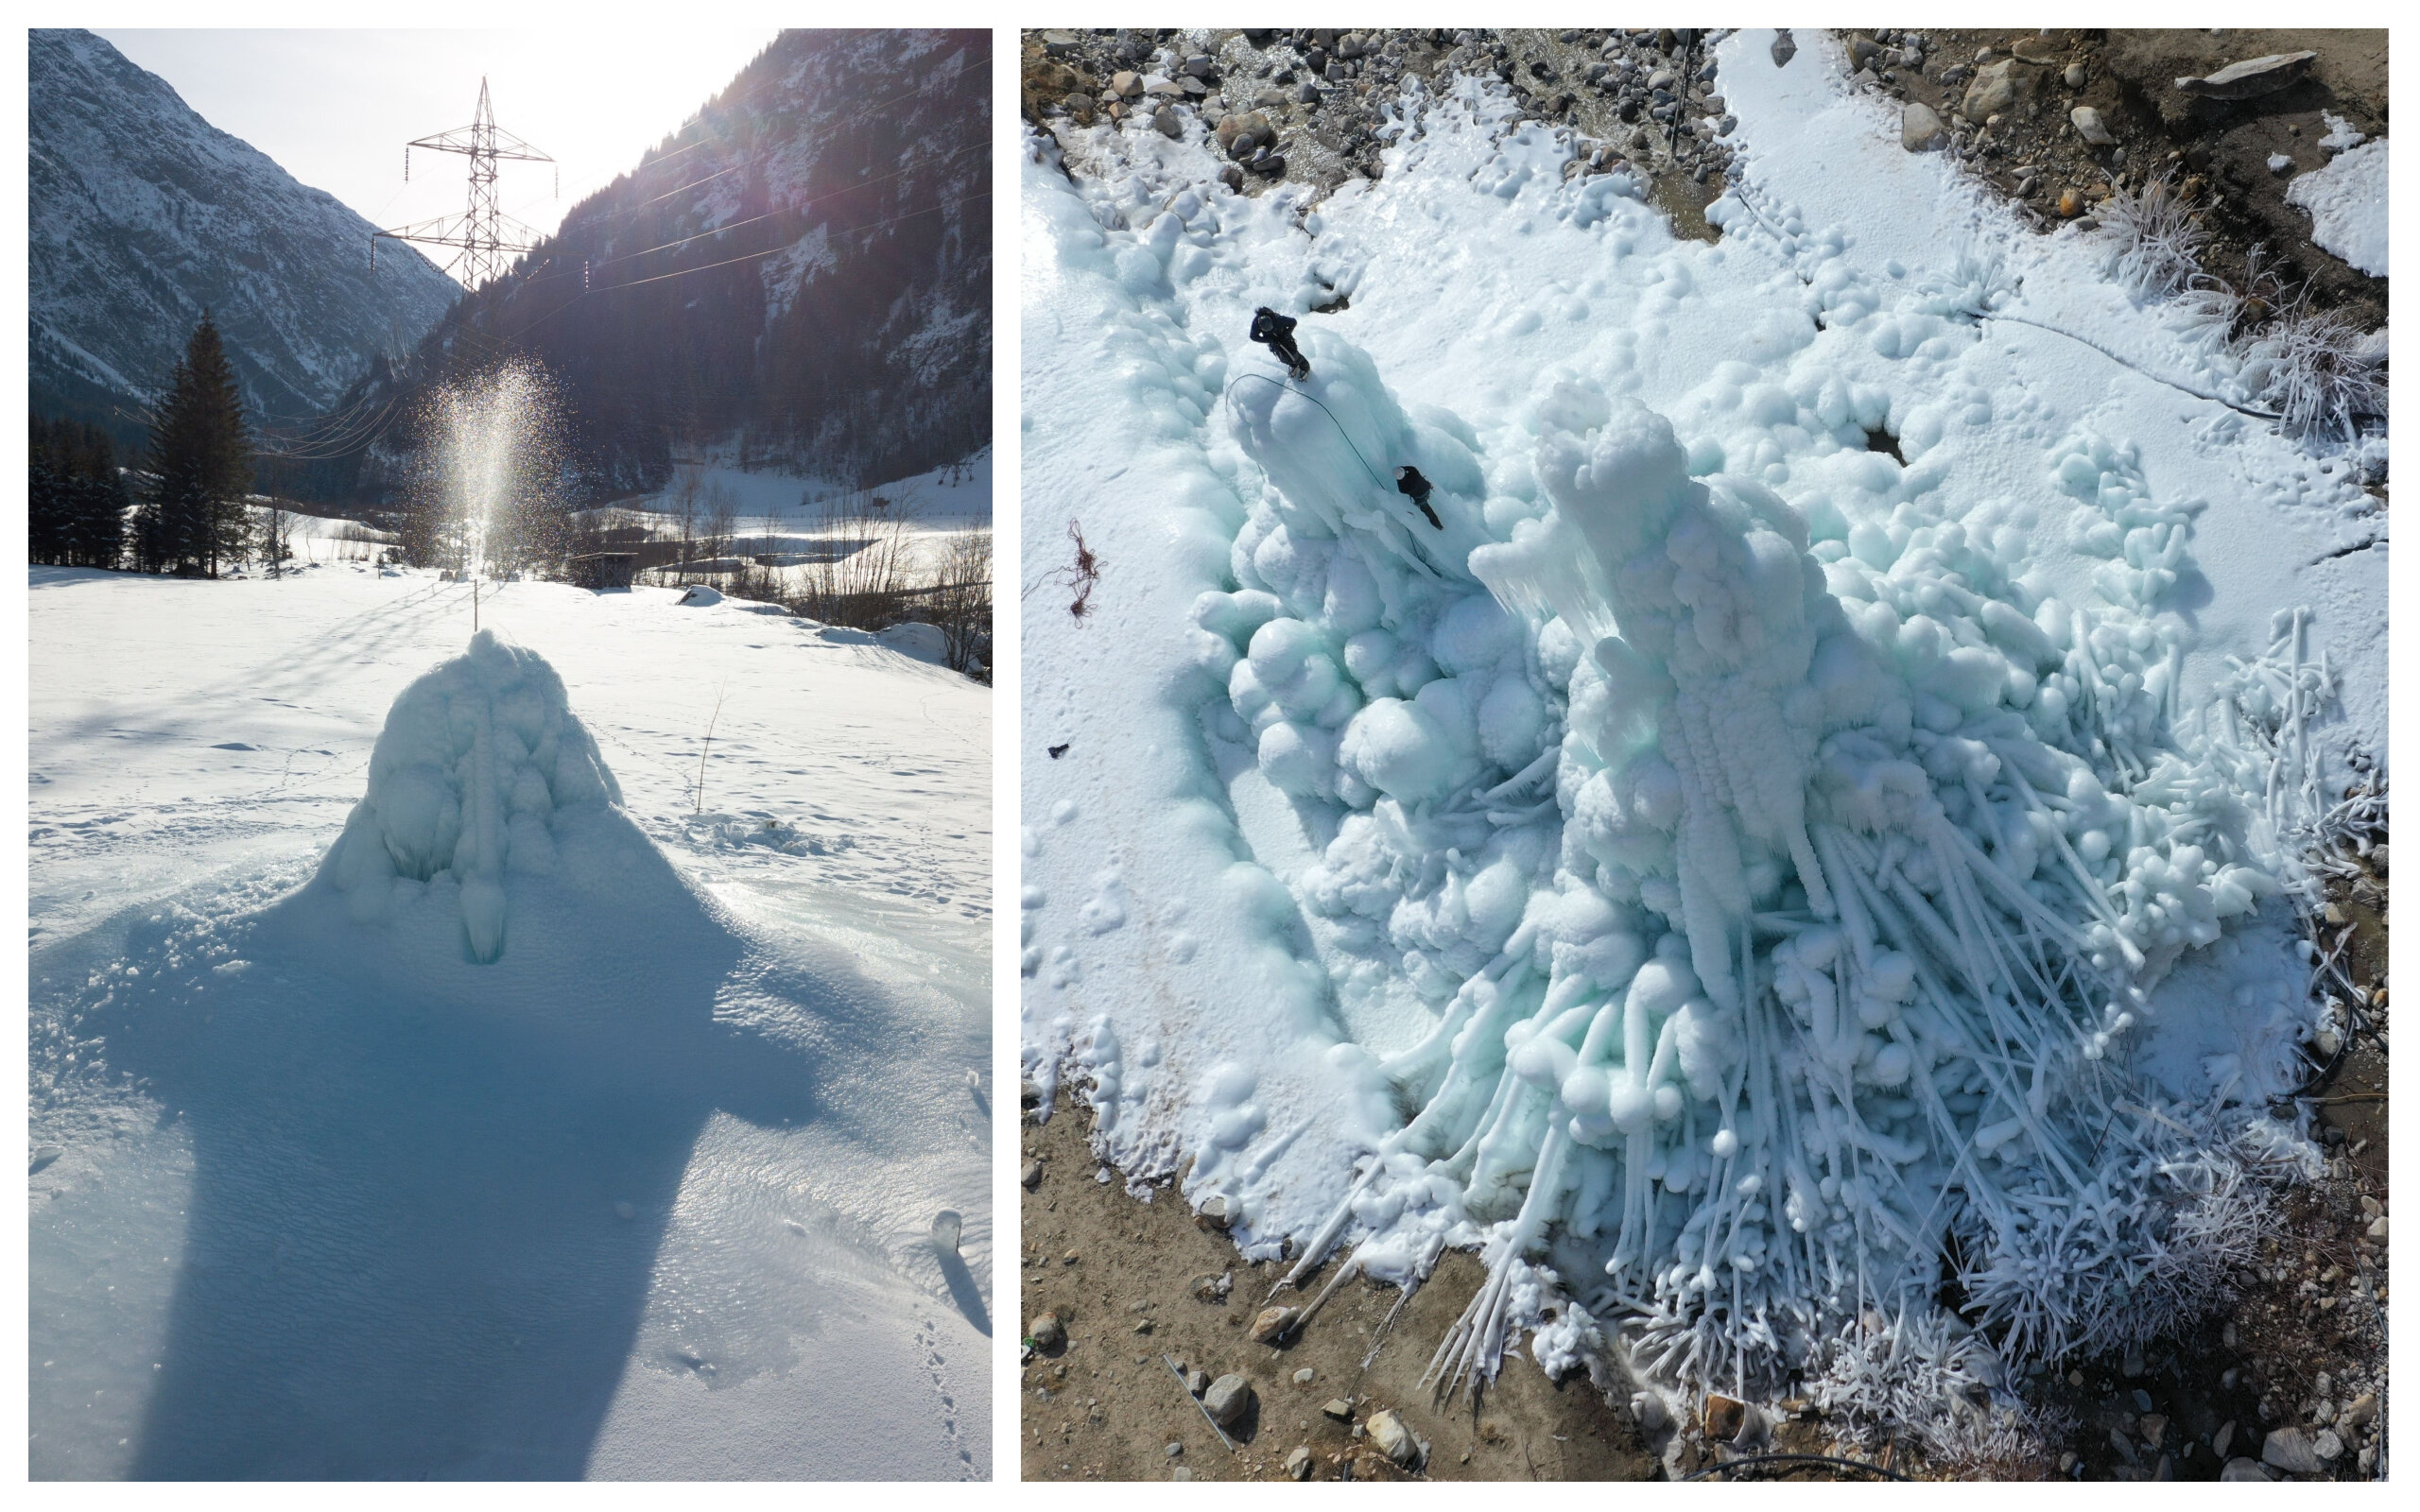
\includegraphics[width=15cm]{./Figures/Figure_2.jpg}
% \caption{(a) The ice structure during the first validation measurement as seen on the webcam image of
%   $14^{th}$ Feb. (b) The corresponding cross section of the EP ice structure with the field estimates of $r, R,
%   h, H_i, H_f$ used to determine the Icestupa volume is shown on the right.} 
%   \label{fig:CH19site} 
%   \end{figure}
% 
% \subsubsection{Weather data}
% Precipitation data was derived from the Plaffeien AWS \citep{meteoswiss} located 8.8 km away from the measurement site
% at an altitude of 1042 $m$ a.s.l.  We recognised during our data analysis that, except precipitation, all the other
% meteorological variables of the EP site correlated much better with the ERA5 dataset than the nearby Plaffeien AWS
% dataset. The $2\,m$ temperature parameter correlated with air temperature ($r^2 =0.9 $), surface pressure parameter
% correlated with air pressure ($r^2 = 1$) and 10m wind speed parameter (derived from horizontal and vertical components)
% correlated with wind speed ($r^2 =0.6 $) .
% 
% Due to a power failure, all data from the EP AWS was lost from $27^{th}$ February 15:20 2019 to $2^{nd}$ March 15:00
% 2019 (equivalent to around 7\% of the measurement period). During heavy snowfall events, the ultrasonic wind sensor was
% blocked and recorded zero values. ERA5 was used to fill such errors and data gaps .
% 
% The ERA5 grid point chosen (Latitude 46° 38' 24" N, Longitude 7° 14' 24" E) for the EP site was around 9 km away from
% the actual site. Near-surface humidity is not provided directly in ERA5 dataset, but from near-surface ($2\,m$ from the
% surface) temperature ($T_{ERA5}$) and dew point temperature ($Tw_{ERA5}$) the relative humidity ($RH$) at $2\,m$  was
% calculated as: 
% 
% \begin{equation} RH = 100 \cdot
%     \frac{e_{sat}(Tw_{ERA5})}{e_{sat}(T_{ERA5})} \end{equation} 
% 
% where the saturation vapour pressure function $e_{sat}$ is expressed with the Teten's formula \citep{Tetens}:
% \begin{equation} e_{sat}(T)= a_1 \cdot e^{(a_3 \cdot \frac{T}{(T+273.16-a_4)})} \end{equation} with T in $\degree C$ and
% the parameters set for saturation over water ($a_1$ = 611.21 Pa, $a_3$ = 17.502 and $a_4$= 32.19 K) according to
% \cite{Buck_1981}.    
% 
% All the ERA5 variables were therefore fitted with the EP dataset via linear regressions.  With the modified ERA5
% dataset, we were also able to further extend the EP dataset and allow the model to run beyond $18^{th}$ March 2019.
% Precipitation was filled as null values beyond $18^{th}$ March 2019.
% 
% \subsubsection{Fountain spray radius of CH19 AIR} \label{section:sprayCH19} 
% This fountain spray radius is determined by modelling the projectile motion of the water droplets. Using mass
% conservation, the droplet speed $v_F$ can be determined from the spray rate $d_F$ and the diameter $dia_F$ of the nozzle
% as follows:
% 
% \begin{equation} v_F = \frac{d_F}{\pi \cdot dia_F^2/4} \end{equation}
% 
% Afterwards, we assume that the water droplets move with an air friction free projectile motion from the fountain
% nozzle with a height $h_F$ to the ice/ground surface. The resulting spray radius $r_F$ was then determined from the
% projectile motion equation as follows:
% 
% \begin{equation} r_F = \frac{v_F \cdot cos\theta_F (v_F \cdot sin\theta_F + \sqrt{(v_F \cdot sin\theta_F)^{2} + 2
% \cdot g \cdot h_F})}{g} \end{equation}
% 
% where $g = 9.8\, m s^{-2}$ is the acceleration due to gravity and $\theta_F$ = 45 $\degree$ is the angle of launch.
% 
% \subsubsection{CH19 Field Measurements for validation} \label{section:validation} 
% The volume was determined by decomposing the ice structure into a cylinder (length $2R$ and height $h$) and a
% cone (radius $r$ and height $(H_i-h)$) through the following equation: 
% \begin{equation} V = \pi \cdot R^2 \cdot h + 1/3 \cdot \pi \cdot r^2 \cdot (H_i-h) \end{equation}
% 
% Manual measurements were performed at the end of the freezing period on $14^{th}$ February 16:00 2019 (only one more
% fountain run was possible after this date) to estimate $r, R, h, H_i, H_f$ (see Fig. \ref{fig:site} for the different
% geometry components):
% 
% $$ 0.55\leq r\leq 1 m\textit{ ; }1.1\leq R\leq 1.2 m\textit{ ; }0.1\leq h\leq 0.2 m\textit{ ; }0.6\leq
% H_i\leq 0.8 m\textit{ ; }1.3\leq H_f\leq 1.4 m  $$
% 
% The ranges of the variables show the variance of the Icestupa's dimensions across different compass orientations.
% Correspondingly, the volume range estimated for the first validation point was 0.857 $\pm$ 0.186 $m^{3}$ on $14^{th}$
% February 16:00 2019.
% 
% The second validation point corresponds to the end of the melting process on $10^{th}$ March 18:00 2019.  Based on the
% webcam imagery and manual measurement, a thin layer of ice with an observed thickness between 0.01 to 0.06 m could be
% quantified. This results in the volume range for the second validation to be 0.13 $\pm$ 0.09 $m^{3}$ on $11^{th}$ March
% 2019 
% 
% In reality, the EP ice structure was more cylindrical until a height of 0.2\,$m$ and conical afterwards until a
% height of 0.6\,$m$ with a radius of 1.18\,$m$. However, we assume a conical shape of this ice structure in order to
% apply the modelling strategy described below.

% \subsubsection{CH21 and CH20 Surface temperature corrections} \label{section:thermalcam} 
% We discarded some thermal camera temperature measurements due to the following reasons:
% \begin{itemize} 
%     \item Snowfall/fog: Whenever there was snow or thick fog, the thermal image was corrupted. Refer image Jan14 1900 and
% Jan3 800. We used the standard deviation of the pixel temperature to identify these events and remove them from the
% validation dataset. 
% 
% \item Strong sunlight: Usually at noon, especially in end of Feb and March, we observed that ice temperature values were
%     above zero C. We found that again the thermal cam images were corrupted as seen in Mar6 1300. So we removed all
%     temperature values above 0 C.  
% 
% \item Then there were some images that were completely blue and looked corrupted.  We cannot identify the cause here but
%     I filtered them out using the mean of all temperature pixels.
% 
% \end{itemize} 

% 
% The CH19 AIR was constructed by the Eispalast in Schwarzsee, Switzerland. It was contained inside a wooden boundary
% adjacent to a stream. Fountain operation was guided by temperature conditions.  The water spray of the fountain was
% initially adjusted so that most of the water droplets land within the wooden boundary zone. The ice formation was guided
% by adding a metal framework at the ice structure base after the first night of operation.  Several cotton threads were
% tied between the ice structure base and fountain pole for accelerating and further guiding the ice formation process. 

% \section*{Conflict of Interest Statement} The authors declare that the research was conducted in the absence of any
% commercial or financial relationships that could be construed as a potential conflict of interest.
% 
% \section*{Author Contributions} SB wrote the initial version of the manuscript. MH, ML, SW, JO, and FK commented on
% the initial manuscript and helped improve it. SB developed the methodology with inputs from MH. SB performed the
% analysis with support from MH and ML. SB and MH participated in the fieldwork.
% 
% \section*{Funding} This work was supported and funded by the University of Fribourg and by the Swiss Government
% Excellence Scholarship (SB).
% 
% \section*{Acknowledgments} We thank Mr. Adolf Kaeser and Mr. Flavio Catillaz at Eispalast Schwarzsee for their active
% participation in the fieldwork. We would also like to thank Digmesa AG for subsidising their flowmeter used in the
% experiment. We would particularly like to thank the editor Prof. Thomas Schuler and 2 anonymous reviewers who gave us
% important inputs to improve the paper. We also thank Prof. Christian Hauck, Prof. Nanna B. Karlsson and Dr. Andrew
% Tedstone for valuable suggestions that improved the manuscript.
% 
% \section*{Data Availability Statement} The data and code used to produce results and figures will be published at a
% later stage and can, until then, be obtained from the authors upon request.

\bibliographystyle{frontiersinSCNS_ENG_HUMS} \bibliography{references}

\end{document}
